\chapter{Systematic Uncertainties}
\label{chap:Systematics}

For this analysis, we consider the following sources of systematic uncertainties:
%%%%%%%%%%%%%%%%%%%%%%%%%%%%%%%%%%%%%%%%%%%%%%%%%%%%%%%%%%%%%
%%%%%%%%%%%%%%%%%%%%%%%%%%%%%%%%%%%%%%%%%%%%%%%%%%%%%%%%%%%%%
\section{Theoretical Uncertainties}
\label{sec:ThUnc}

\begin{itemize}
\item Prompt background cross-sections: These uncertainties arise from the uncertainties in the measured cross-sections of the processes which are used for scaling the MC to the luminosity of data. Systematic uncertainties associated to the prompt backgrounds WZ ( as discussed in autoref{sec:CRWZ} ), ZZ , ttW/ttZ/ttH, tZq are 6$\%$, 6$\%$, 15$\%$ and 20$\%$ respectively. Measurements performed on the WZ and ZZ processes currently have uncertainties of order 5-8$\%$ cite{WZ2019} cite{ZZ2020}. A 50 $\%$ normalization uncertainty is assigned to other smaller backgrounds.
 \item PDF: Using 100 the replicas of the NNPDF 3.1 set, the PDF uncertainties are obtained by taking the root mean square value of the variations. Only shape components of the variation is considered, this is done by normalizing LHE weights of the replicas such that the sum of the LHE wights (in SR) stays the same for each replica. This uncertainty treated as correlated. We consider this uncertainty for all the signals and major prompt backgrounds (i.e. WZ, TTZ, TTW and TTH).
 \item Renormalization and factorization scale: this uncertainty is evaluated by considering an envelope of 6 variation ($\mu_R$ 2, $\mu_R$ 0.5, $\mu_F$ 2, $\mu_F$ 0.5, $\mu_R$ and $\mu_F$ 2, $\mu_R$ and $\mu_F$ 0.5). This uncertainty is treated as correlated and only shape component is considered. We consider this uncertainty for all the signals and major prompt backgrounds (i.e. WZ, TTZ, TTW and TTH).
 \item ISR and FSR: initial state radiation and final state radiation uncertainty is evaluated by using the default set of variation (2 and 0.5). This uncertainty is treated as correlated and only shape component is considered. We consider this uncertainty for all the signals.
\end{itemize}
%%%%%%%%%%%%%%%%%%%%%%%%%%%%%%%%%%%%%%%%%%%%%%%%%%%%%%%%%%%%%
%%%%%%%%%%%%%%%%%%%%%%%%%%%%%%%%%%%%%%%%%%%%%%%%%%%%%%%%%%%%%
\section{Nonprompt Uncertainties}
\label{sec:NonUnc}

We consider the following sources of systematic uncertainties (shape) associated with the \emph{fake} efficiency.

\begin{itemize}
\item Prompt background correction
\item Sample dependence 
\item Statistical uncertainty 
\end{itemize}

An important systematic uncertainty comes from the estimate of prompt contamination in MR. As is discussed in \autoref{sec:Nonprompt}, prompt backgrounds (estimated with MC) are subtracted from total event yields measured in MR (data). A flat 20 $\%$ uncertainty ($\alpha$ in Equation \ref{eq:f_eq}) is assigned to the event yields of the prompt background and the resulting variation of \emph{f} is taken as the uncertainty, which is estimated to be between 5 $\%$ and 15 $\%$.

\begin{equation}
f=\frac{n_{data}^{T}-(1+\alpha)n_{Prompt~MC}^{T}}{n_{data}^{T+\overline{T}}-(1+\alpha)n_{Prompt~MC}^{T+\overline{T}}}.
\label{eq:f_eq}
\end{equation}  

\begin{figure}[tbh!]
 \begin{center}
 \begin{tabular}{c}
 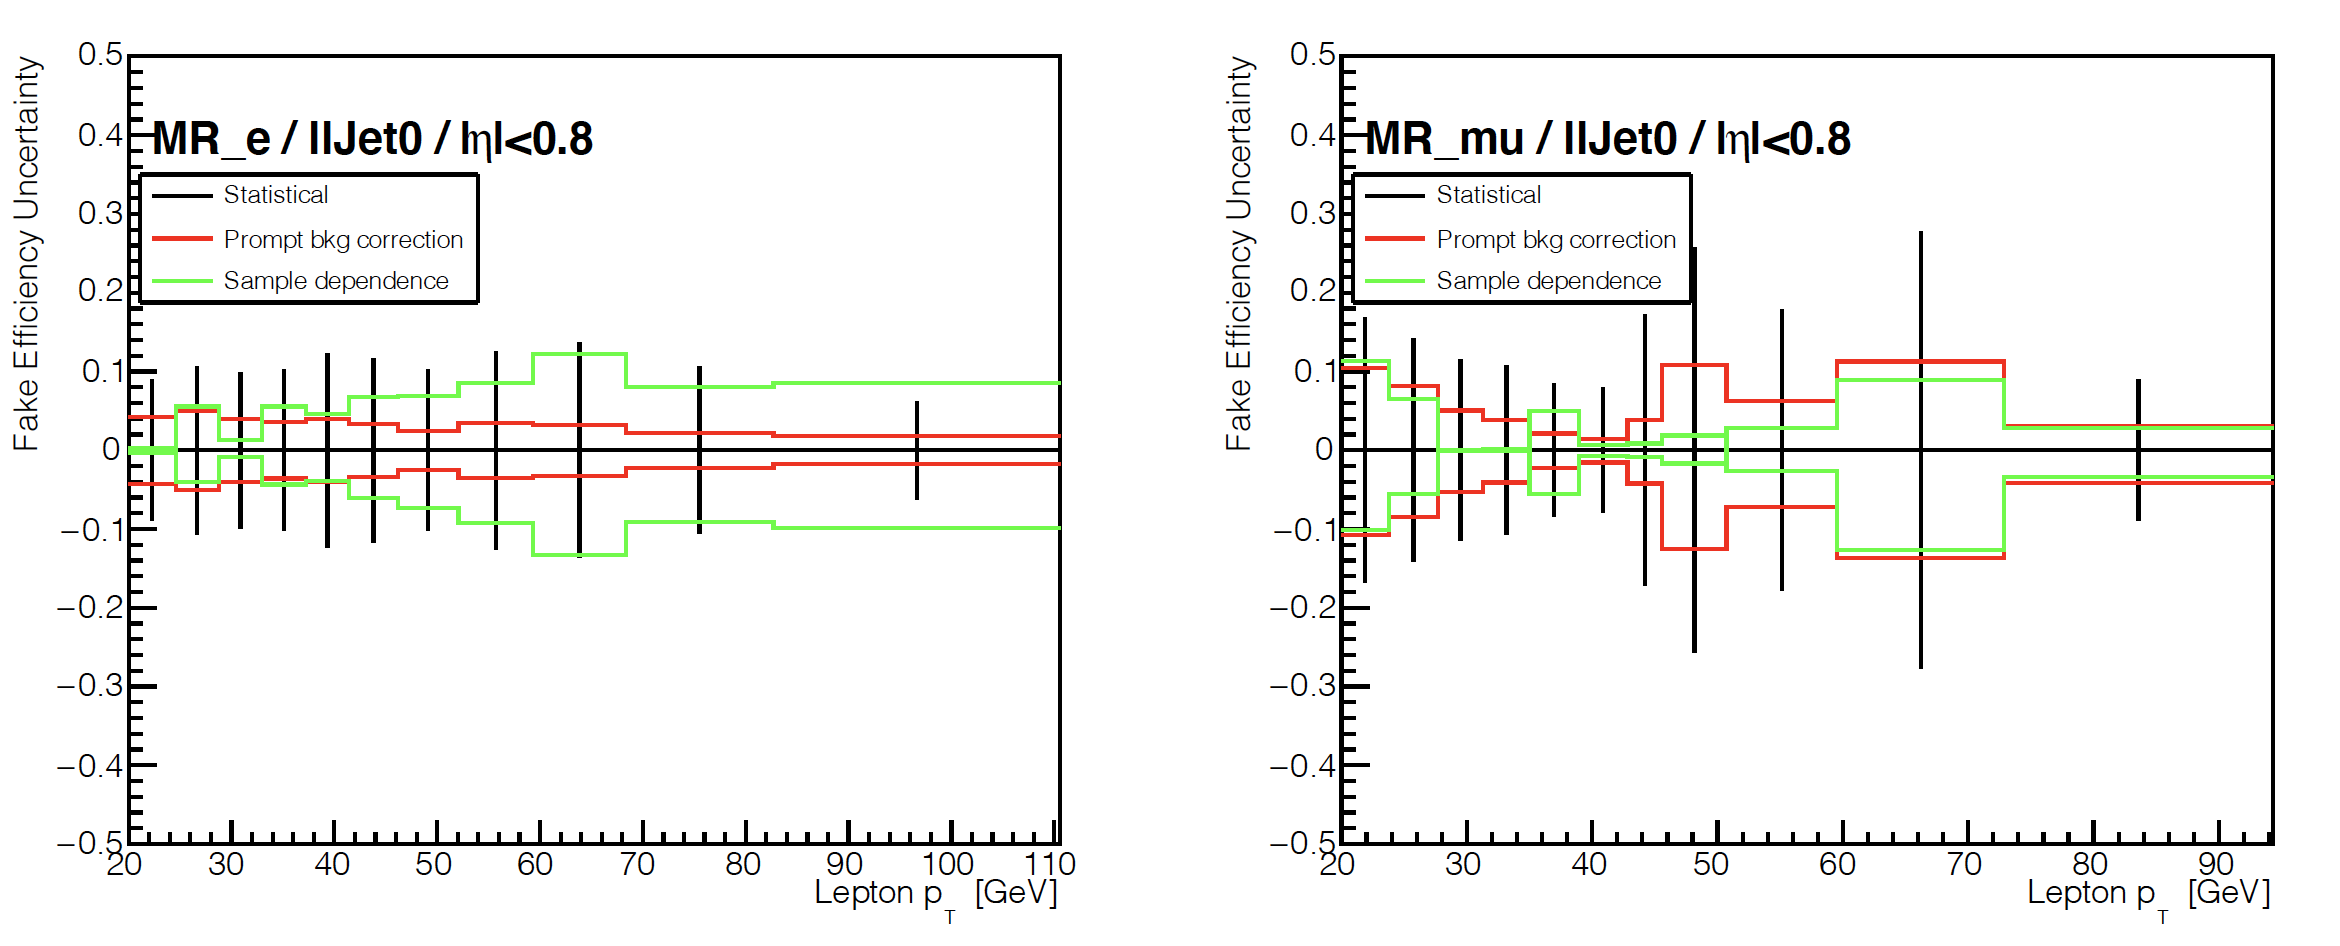
\includegraphics[width=0.99\textwidth]{figures/Part3/Systematics/MR1}
 \end{tabular}
 \caption{Comparison of different components of the uncertainties associated to the \emph{fake} efficiency measured in 2017 dataset (njet=0 bin, $|\eta|<$0.8 bin). From left to right: electron \emph{f} uncertainty, muon \emph{f} uncertainty. Note: black uncertainty bars represent statistical uncertainties.}
 \label{fig:f_comp1}
 \end{center}
\end{figure}

Sample dependence is one of the primary sources of systematic uncertainty and it is concerned with the possibility that the \emph{fake} efficiency \emph{f} measured in MR may not reflect characteristics of the non-prompt leptons in SR due to different compositions of backgrounds. This type of uncertainty is estimated by introducing a variation factor $\beta$ between the proportions of Same-Flavor and Opposite-Flavor pairs in MR. For example, electron \emph{f} can be calculated as (prompt background correction is ignored from the equation): 

\begin{equation}
f_{e}=\frac{(1+\beta)n_{F,e+e}^{T}+(1-\beta)n_{F,e+\mu}^{T}}{(1+\beta)n_{F,e+e}^{T+\overline{T}}+(1-\beta)n_{F,e+\mu}^{T+\overline{T}}}.
 \label{eq:samp_dep}
\end{equation}

A 20$\%$ variation ($\beta$) is assigned the resulting variation of \emph{f} is taken as the uncertainty, which is estimated to be between 3 $\%$ and 15 $\%$. 
 
A comparison of different sources of systematic uncertainties (using 2017 datasets) are shown in Figure \ref{fig:f_comp1} and Figure \ref{fig:f_comp2}. A complete summary of uncertainties associated to \emph{real} and \emph{fake} efficiency can be found in.

\begin{figure}[tbh!]
 \begin{center}
 \begin{tabular}{c}
 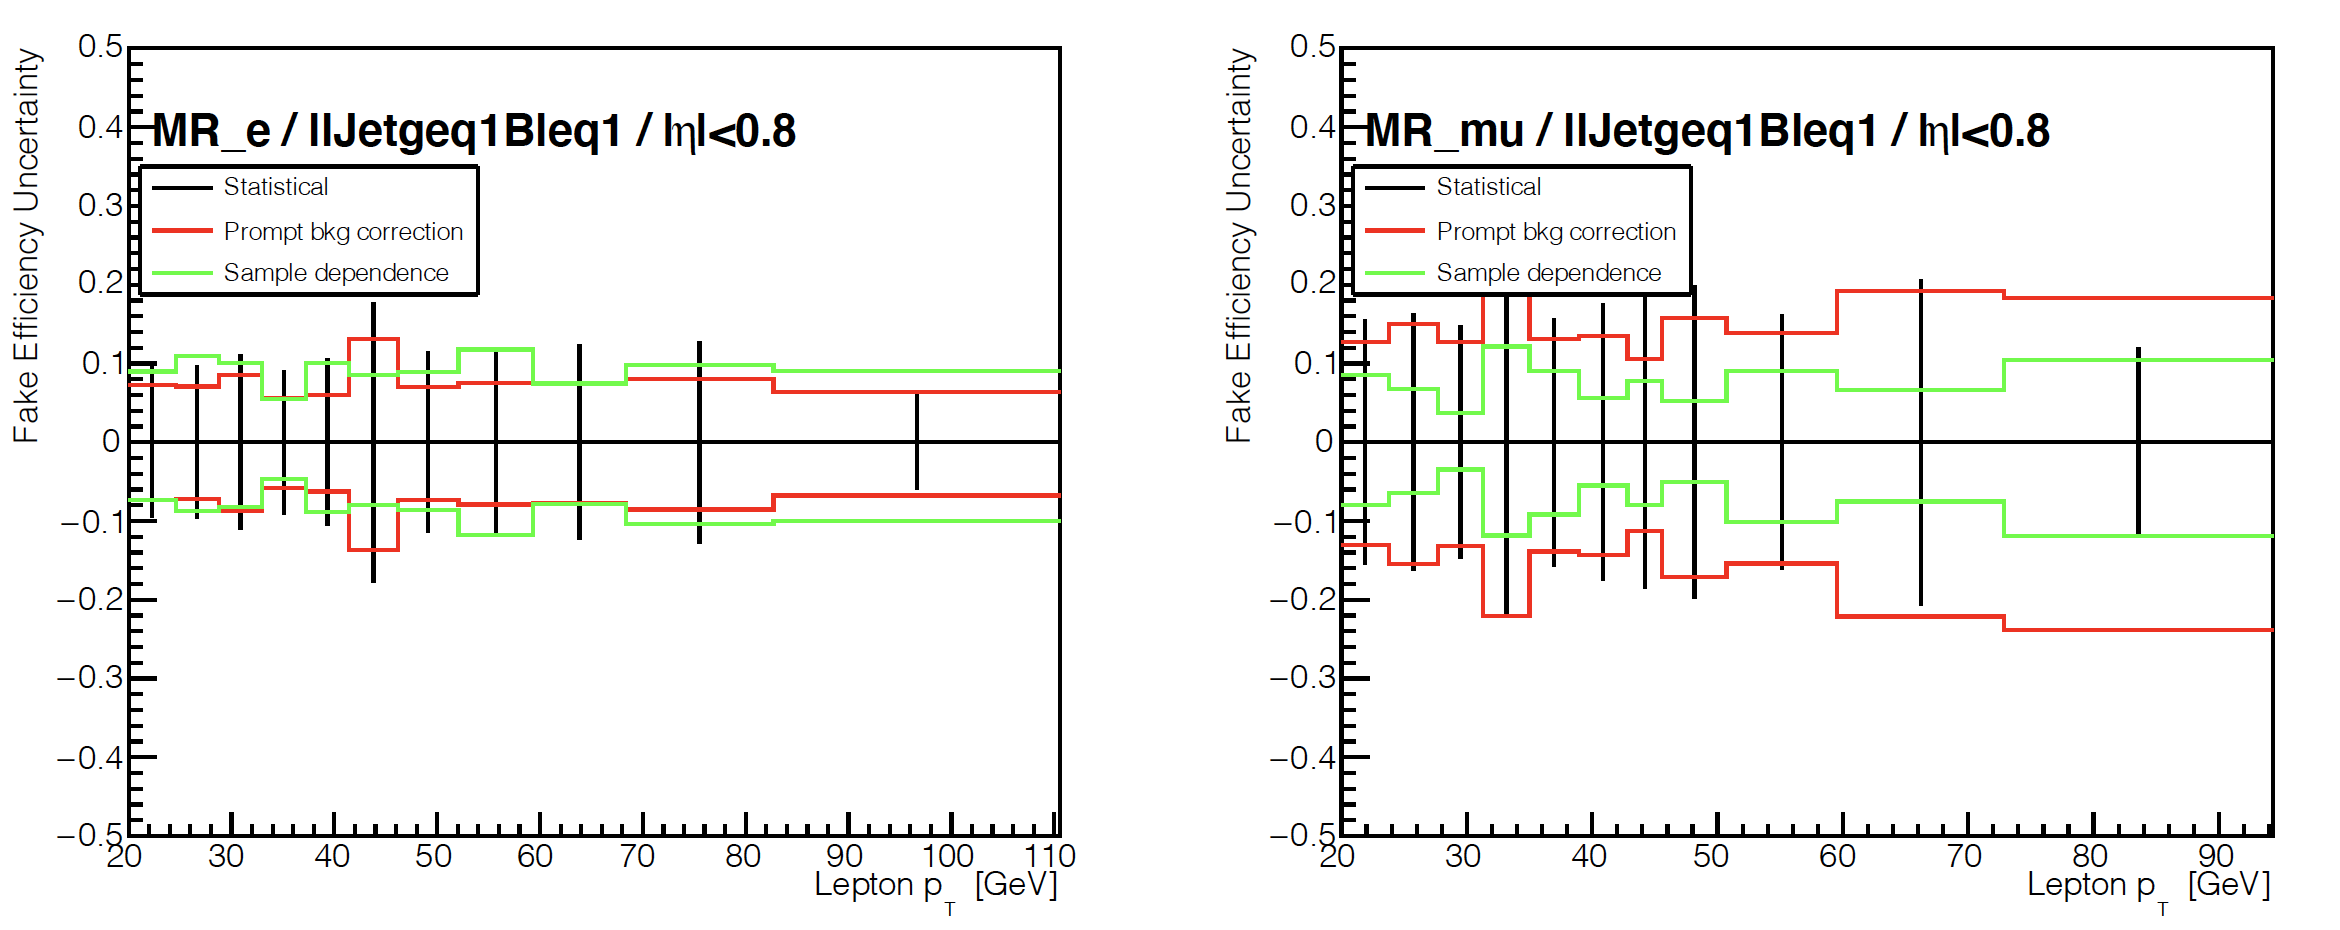
\includegraphics[width=0.99\textwidth]{figures/Part3/Systematics/MR2}
 \end{tabular}
 \caption{Comparison of different components of the uncertainties associated to the \emph{fake} efficiency measured in 2017 dataset (njet$>$0 bin, $|\eta|<$0.8 bin). From left to right: electron \emph{f} uncertainty, muon \emph{f} uncertainty. Note: black uncertainty bars represent statistical uncertainties.}
 \label{fig:f_comp2}
 \end{center}
\end{figure}

In addition to statistical uncertainties, MC uncertainties are propagated to the \emph{real} efficiency as sources of systematic uncertainties:

\begin{itemize}
\item Statistical uncertainty 
\item MC uncertainty 
\begin{itemize}
\item Electron reconstruction 
\item b-tagging 
\item JES/JER
\item Pile-up rewighting 
\item ECAL prefiring 
\end{itemize}
\end{itemize}

The uncertainties associated to the \emph{real} efficiency are relatively small when compared to the \emph{fake} efficiency uncertainties. A comparison of different sources of \emph{real} efficiency uncertainties are shown in Figure \ref{fig:r_comp}.

\begin{figure}[tbh!]
 \begin{center}
 \begin{tabular}{c}
 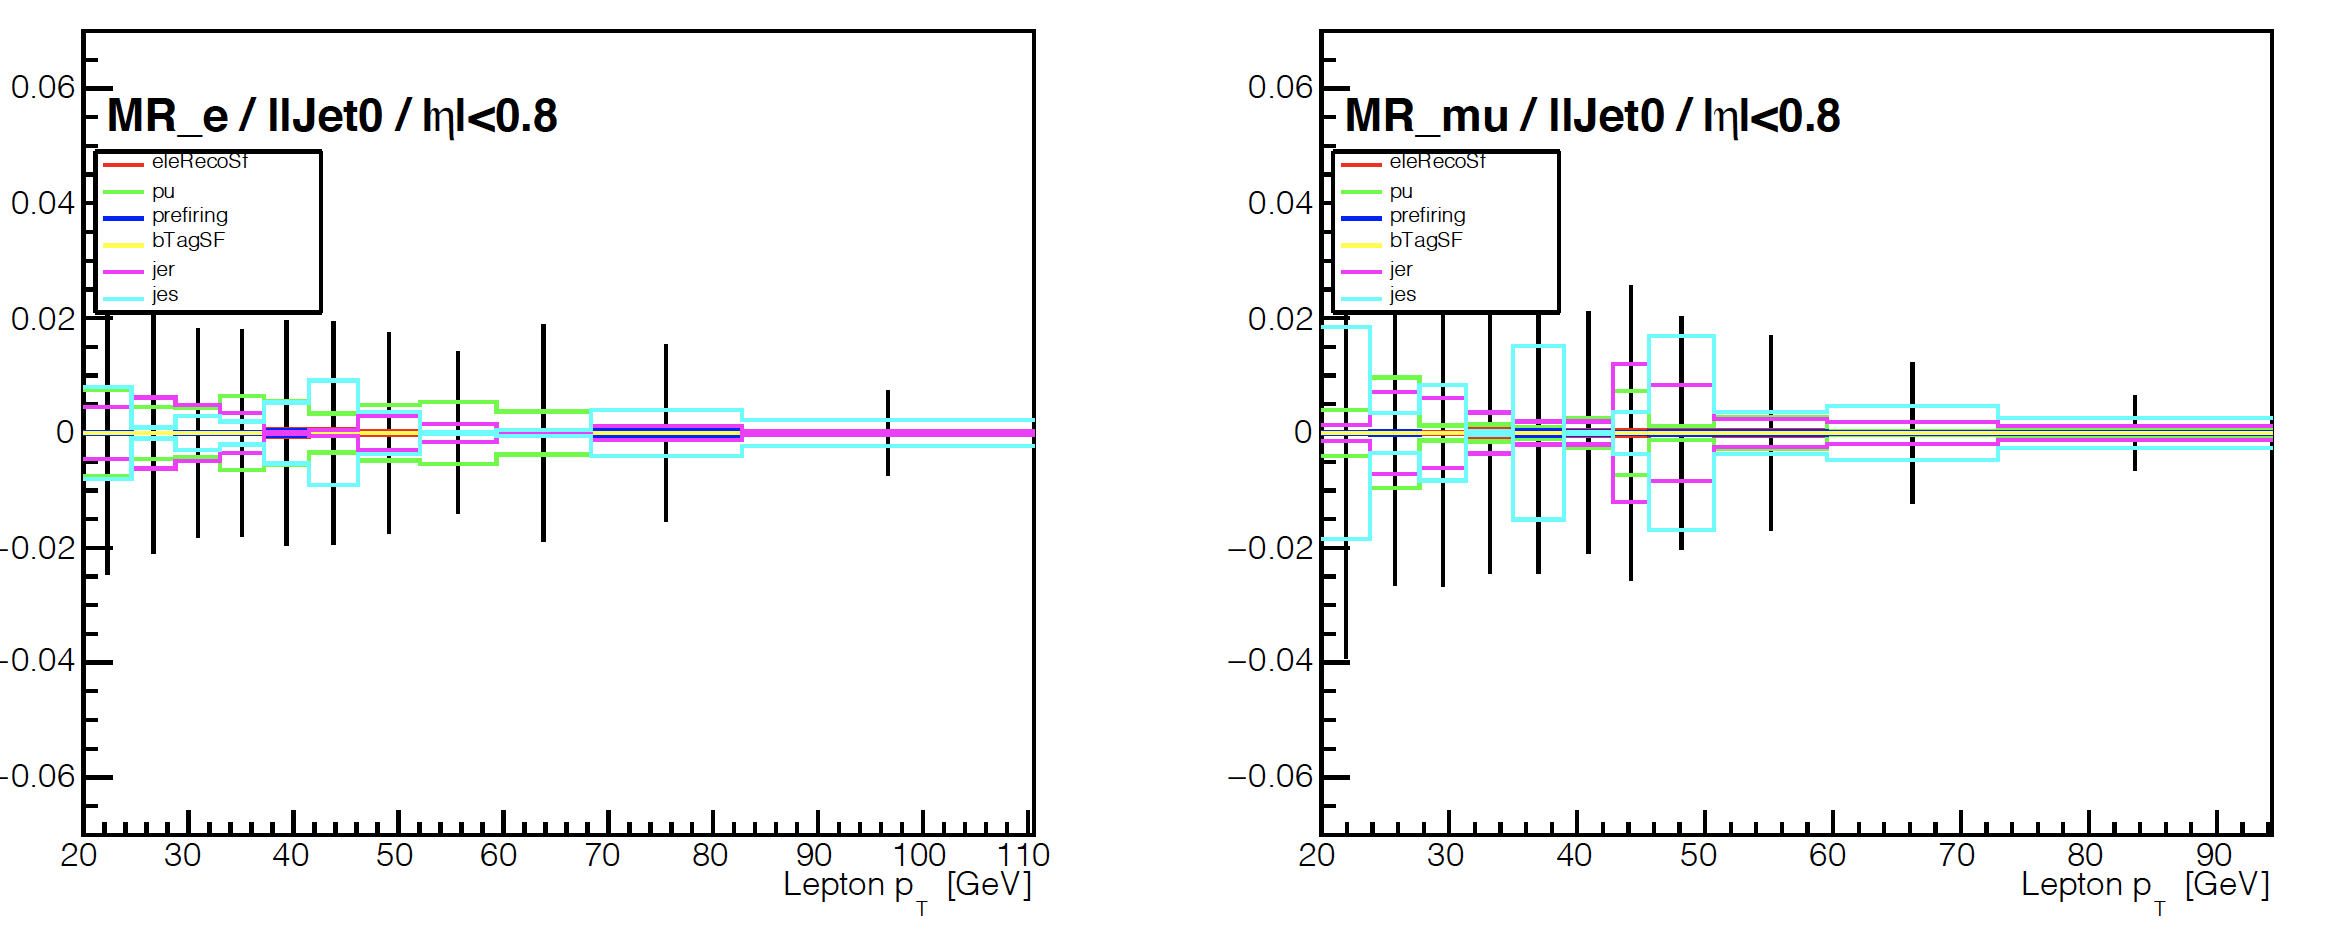
\includegraphics[width=0.99\textwidth]{figures/Part3/Systematics/MR}
 \end{tabular}
 \caption{Comparison of different components of the uncertainties associated to the \emph{real} efficiency measured in 2017 dataset (njet$=$0 bin, $|\eta|<$0.8 bin). From left to right: electron \emph{r} uncertainty, muon \emph{r} uncertainty. Note: black uncertainty bars represent statistical uncertainties.}
 \label{fig:r_comp}
 \end{center}
\end{figure}

In addition to the four components (i.e. $r_e$, $r_{\mu}$, $f_e$, $f_{\mu}$) of the shape uncertainties associated to the measurement of $r$ and $f$, a fifth component is considered that accounts for the potential bias introduced when implementing 3D matrix method: Four out of the eight regions that appear on the lefthand side of the Equation \ref{eq:matrix_method3} (i.e. $N^{\overline{T}TT}$, $N^{\overline{T}T\overline{T}}$, $N^{\overline{T}\overline{T}T}$, $N^{\overline{T}\overline{T}\overline{T}}$) are selected by requiring the leading lepton to fail the \emph{tight} criteria (See Table \ref{tab:looseandtight}). Effectively this means that the isolation requirement is reversed for leading lepton that enter these four regions. Selecting the leading lepton by a loose/reversed isolation requirement is not ideal since the leading lepton is required to match with iso-trigger. To account for this bias, a 50 $\%$ uncertainty is assigned to the $f_1$ (\emph{fake} efficiency of the leading lepton) for events that enter these four regions. The variation of the non-prompt estimate due to trigger matching is largely covered by this uncertainty (See Figure \ref{fig:MM_trigger}).

\begin{figure}[tbh!]
 \begin{center}
 \begin{tabular}{cc}
 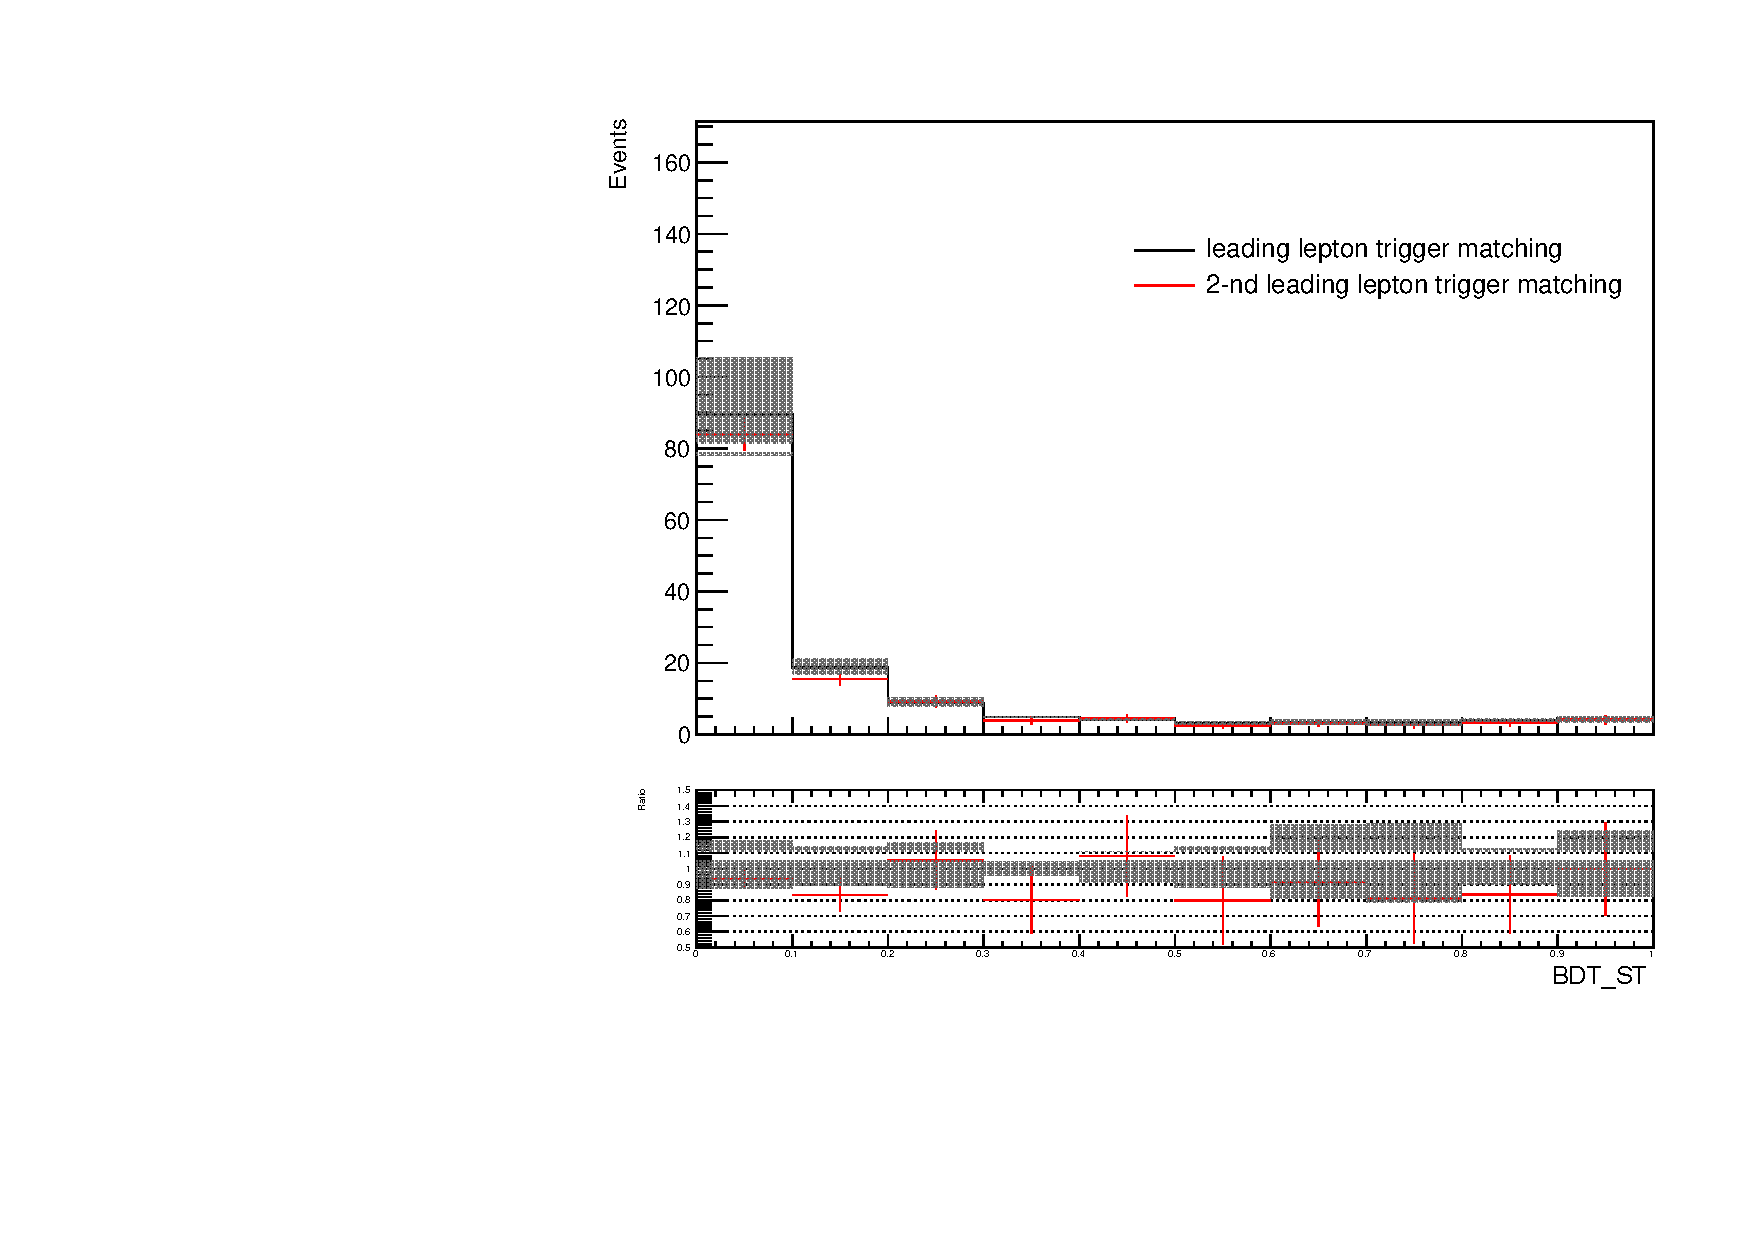
\includegraphics[width=0.47\textwidth]{figures/Part3/Systematics/BDT_ST_MM}&
 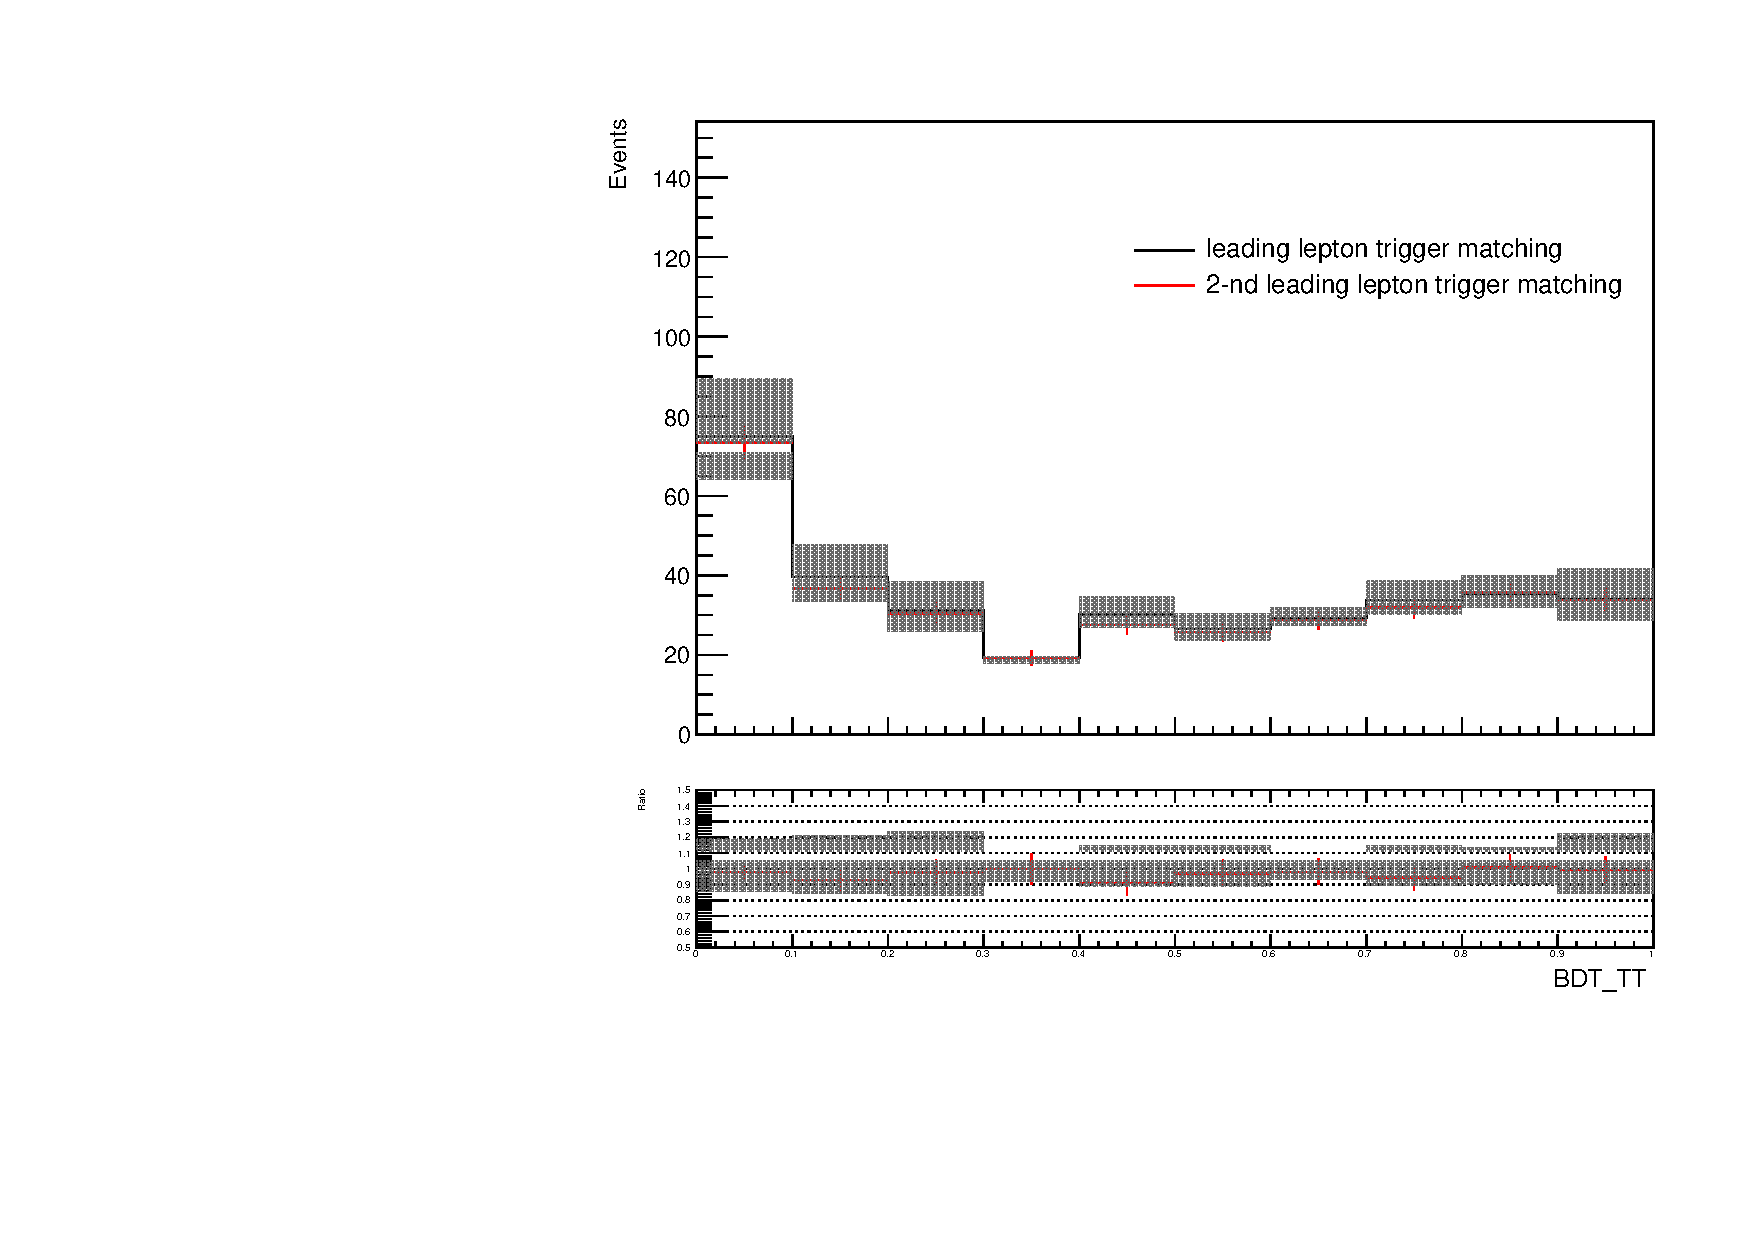
\includegraphics[width=0.47\textwidth]{figures/Part3/Systematics/BDT_TT_MM} \\
 \end{tabular}
 \caption{The impact of matching leptons to trigger objects on non-prompt estimate. From left to right: non-prompt estimate in ST enriched SR, non-prompt estimate in TT enriched SR. The nominal configuration of the matrix method is to match the leading lepton with trigger objects. Matching the 2nd-leading with the trigger objects is taken as an alternative to evaluate the robustness of the non-prompt estimate. The uncertainty band only covers the variation of the non-prompt estimate as a result of varying leading lepton $f$ by 50 $\%$. Uncertainty bars only include statistical uncertainties.}
 \label{fig:MM_trigger}
 \end{center}
\end{figure}

The five components of the uncertainties discussed in this section are propagated through the matrix inversion. The resulting variations of the non-prompt estimates are taken as the shape uncertainties assigned to non-prompt backgrounds. These uncertainties are treated as correlated between the years. In addition to these shape uncertainties, an overall normalization uncertainty of 10$\%$ is assigned in order to cover any other potential bias.
%%%%%%%%%%%%%%%%%%%%%%%%%%%%%%%%%%%%%%%%%%%%%%%%%%%%%%%%%%%%%
%%%%%%%%%%%%%%%%%%%%%%%%%%%%%%%%%%%%%%%%%%%%%%%%%%%%%%%%%%%%%
\section{Diboson Uncertainties}
\label{sec:DiUnc}

Mismodeling of the jet multiplicity is observed in WZ control region (See autoref{sec:CRWZ}). This is largely due to the fact that jets generated from diboson samples are coming from radiation (due to our trilepton selection). Therefore, the accuracy of the jet multiplicity distribution is suboptimal. To take this into account, a dedicated jet-dependent uncertainty is assigned to each event. This uncertainty is determined using diboson control region:

\begin{itemize}
\item Exactly three leptons (any flavor composite),
\item OnZ,
\item MET$>$85GeV,
\item Veto events with at least one b-tag jet ($p_T>$20GeV).
\end{itemize}

The jet multiplicity distributions are shown in Figure \ref{fig:VV_CR}. For each year, a scale factor parameterized as bins of jet multiplicity is derived:

\begin{equation}
\epsilon=\frac{N_{data}-N_{VVV}-N_{TX}-N_{TTbar}-N_{others}}{N_{VV}}.
\end{equation}

\begin{figure}[tbh!]
 \begin{center}
 \begin{tabular}{ccc}
  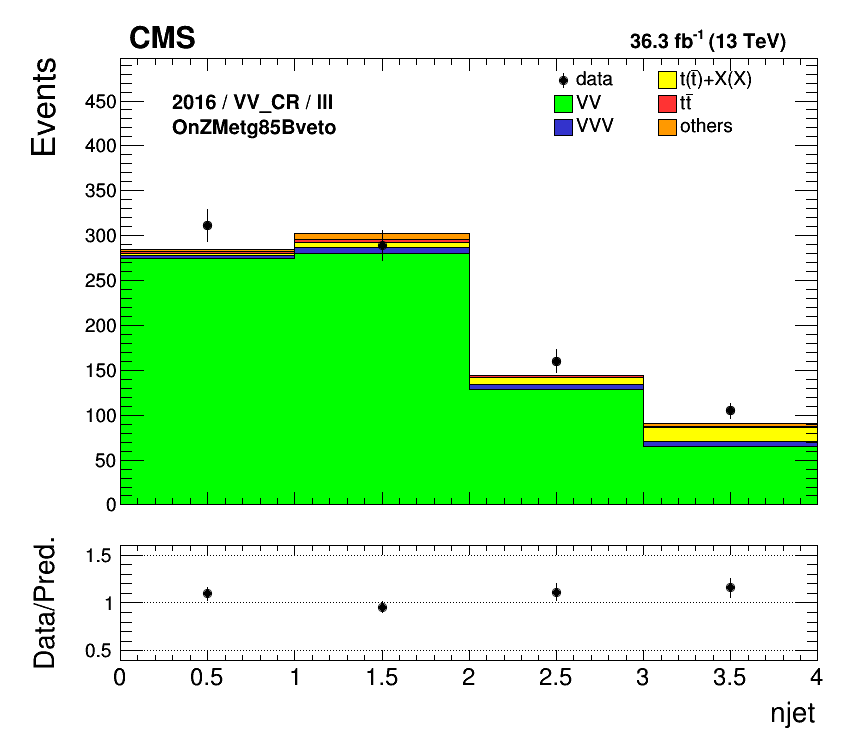
\includegraphics[width=0.325\textwidth]{figures/Part3/Systematics/njet_2016}&
    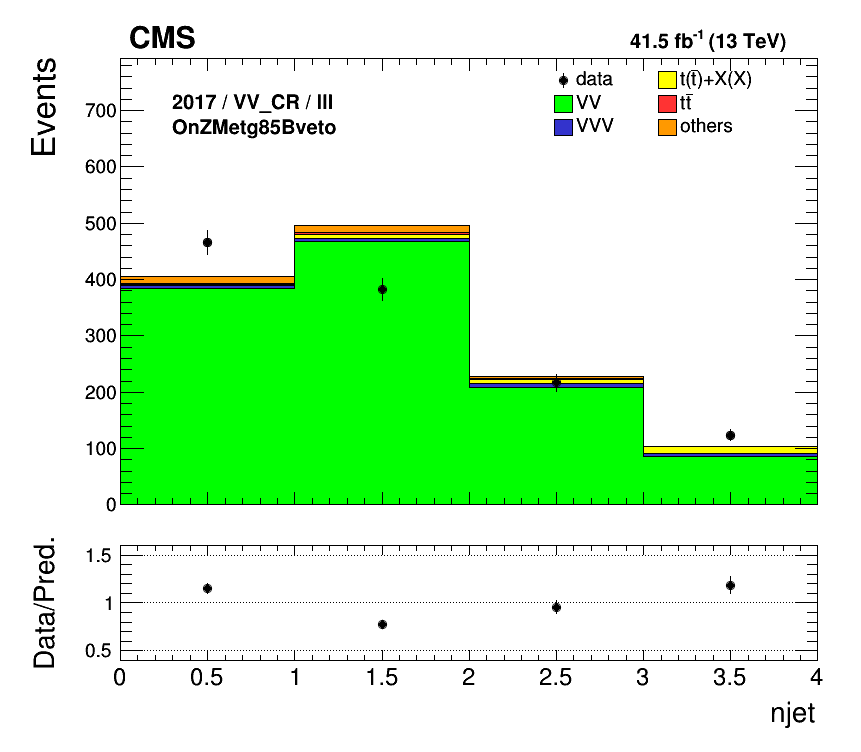
\includegraphics[width=0.325\textwidth]{figures/Part3/Systematics/njet_2017}&
  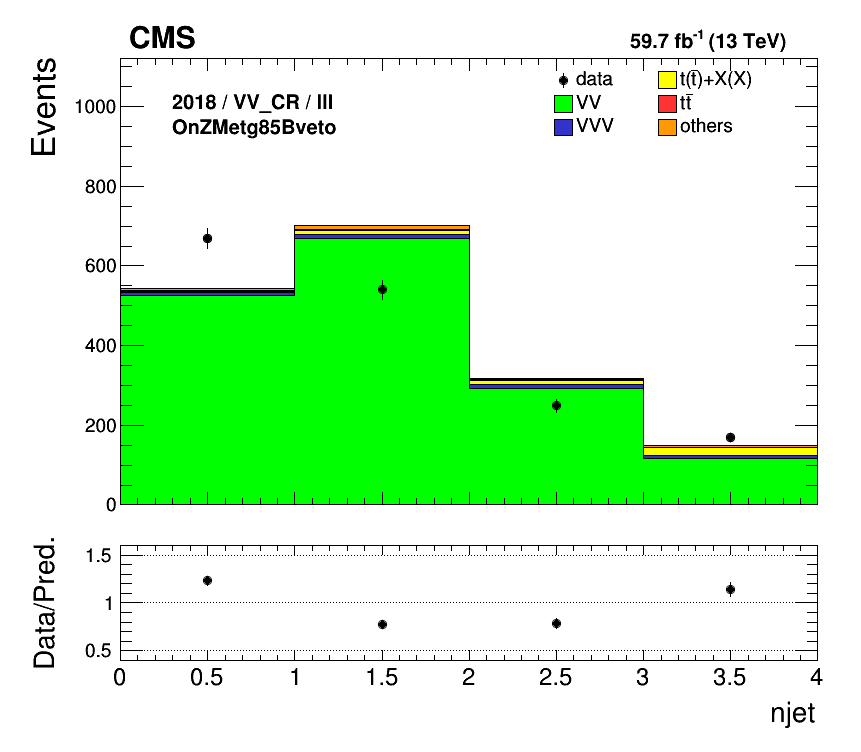
\includegraphics[width=0.325\textwidth]{figures/Part3/Systematics/njet_2018}\\
 \end{tabular}
 \caption{Diboson control region, from left to right: 2016, 2017 and 2018 datasets.}
 \label{fig:VV_CR}
 \end{center}
\end{figure}

The scale factor $\epsilon$ is used to estimate the uncertainty, denoted by $\Delta$:

\begin{equation}
\Delta=|1-\epsilon|
\end{equation}

\begin{figure}[tbh!]
 \begin{center}
 \begin{tabular}{ccc}
  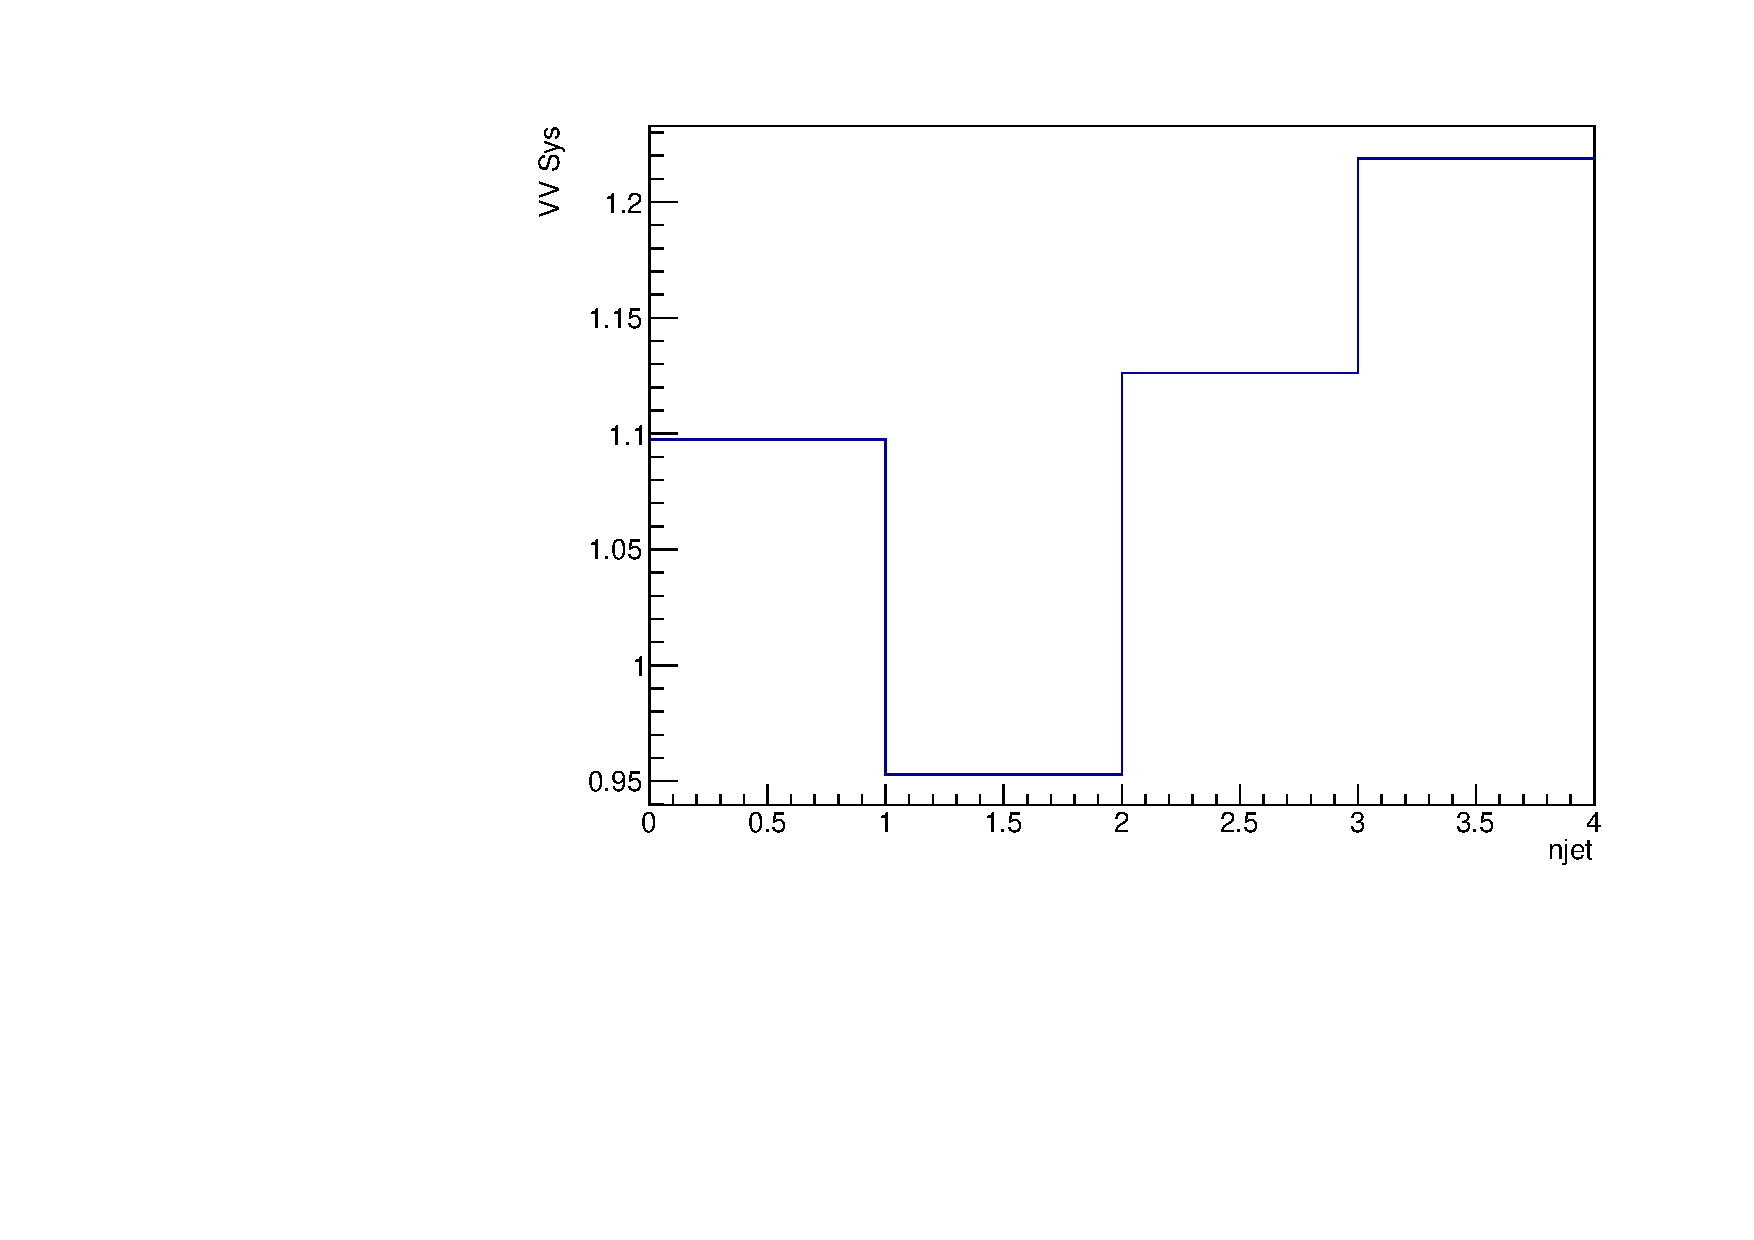
\includegraphics[width=0.325\textwidth]{figures/Part3/Systematics/2016_VV_Sys_1D}&
    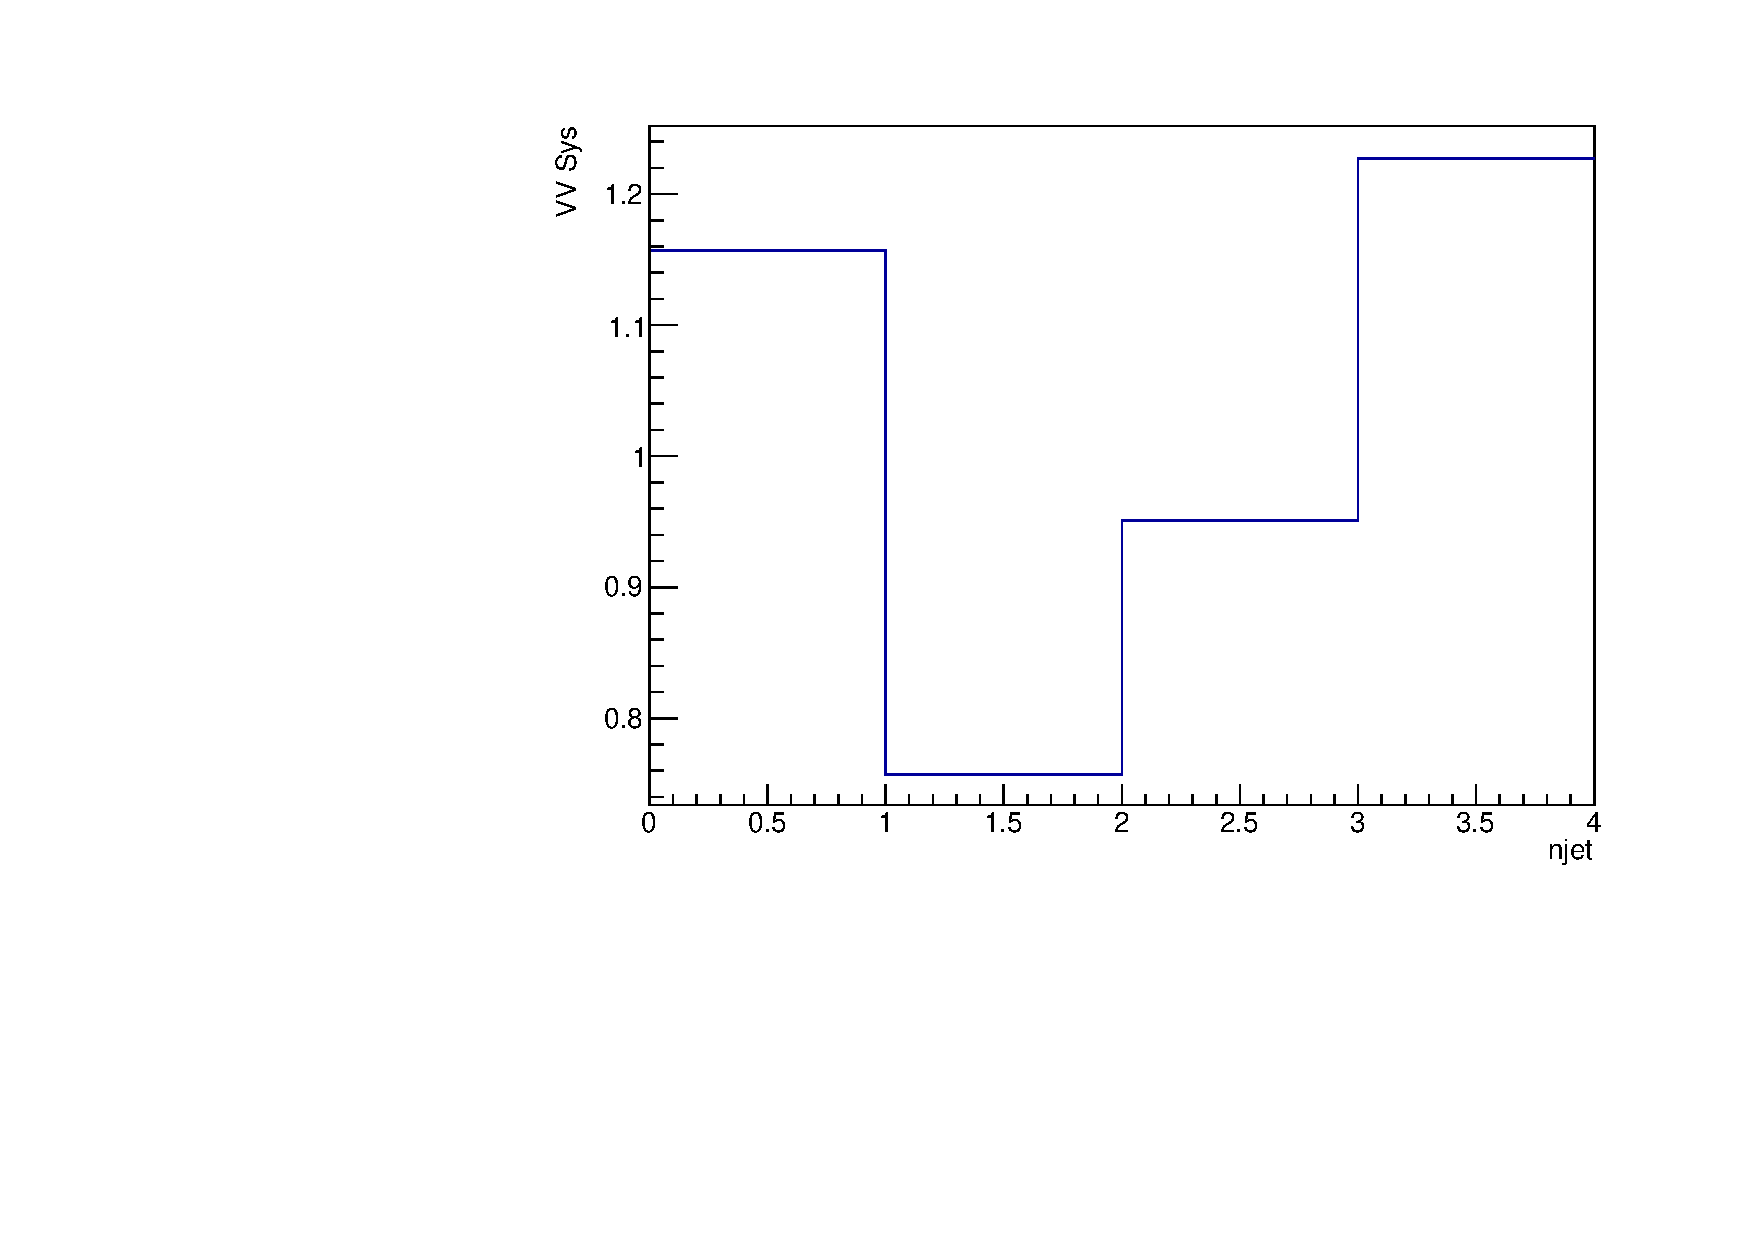
\includegraphics[width=0.325\textwidth]{figures/Part3/Systematics/2017_VV_Sys_1D}&
  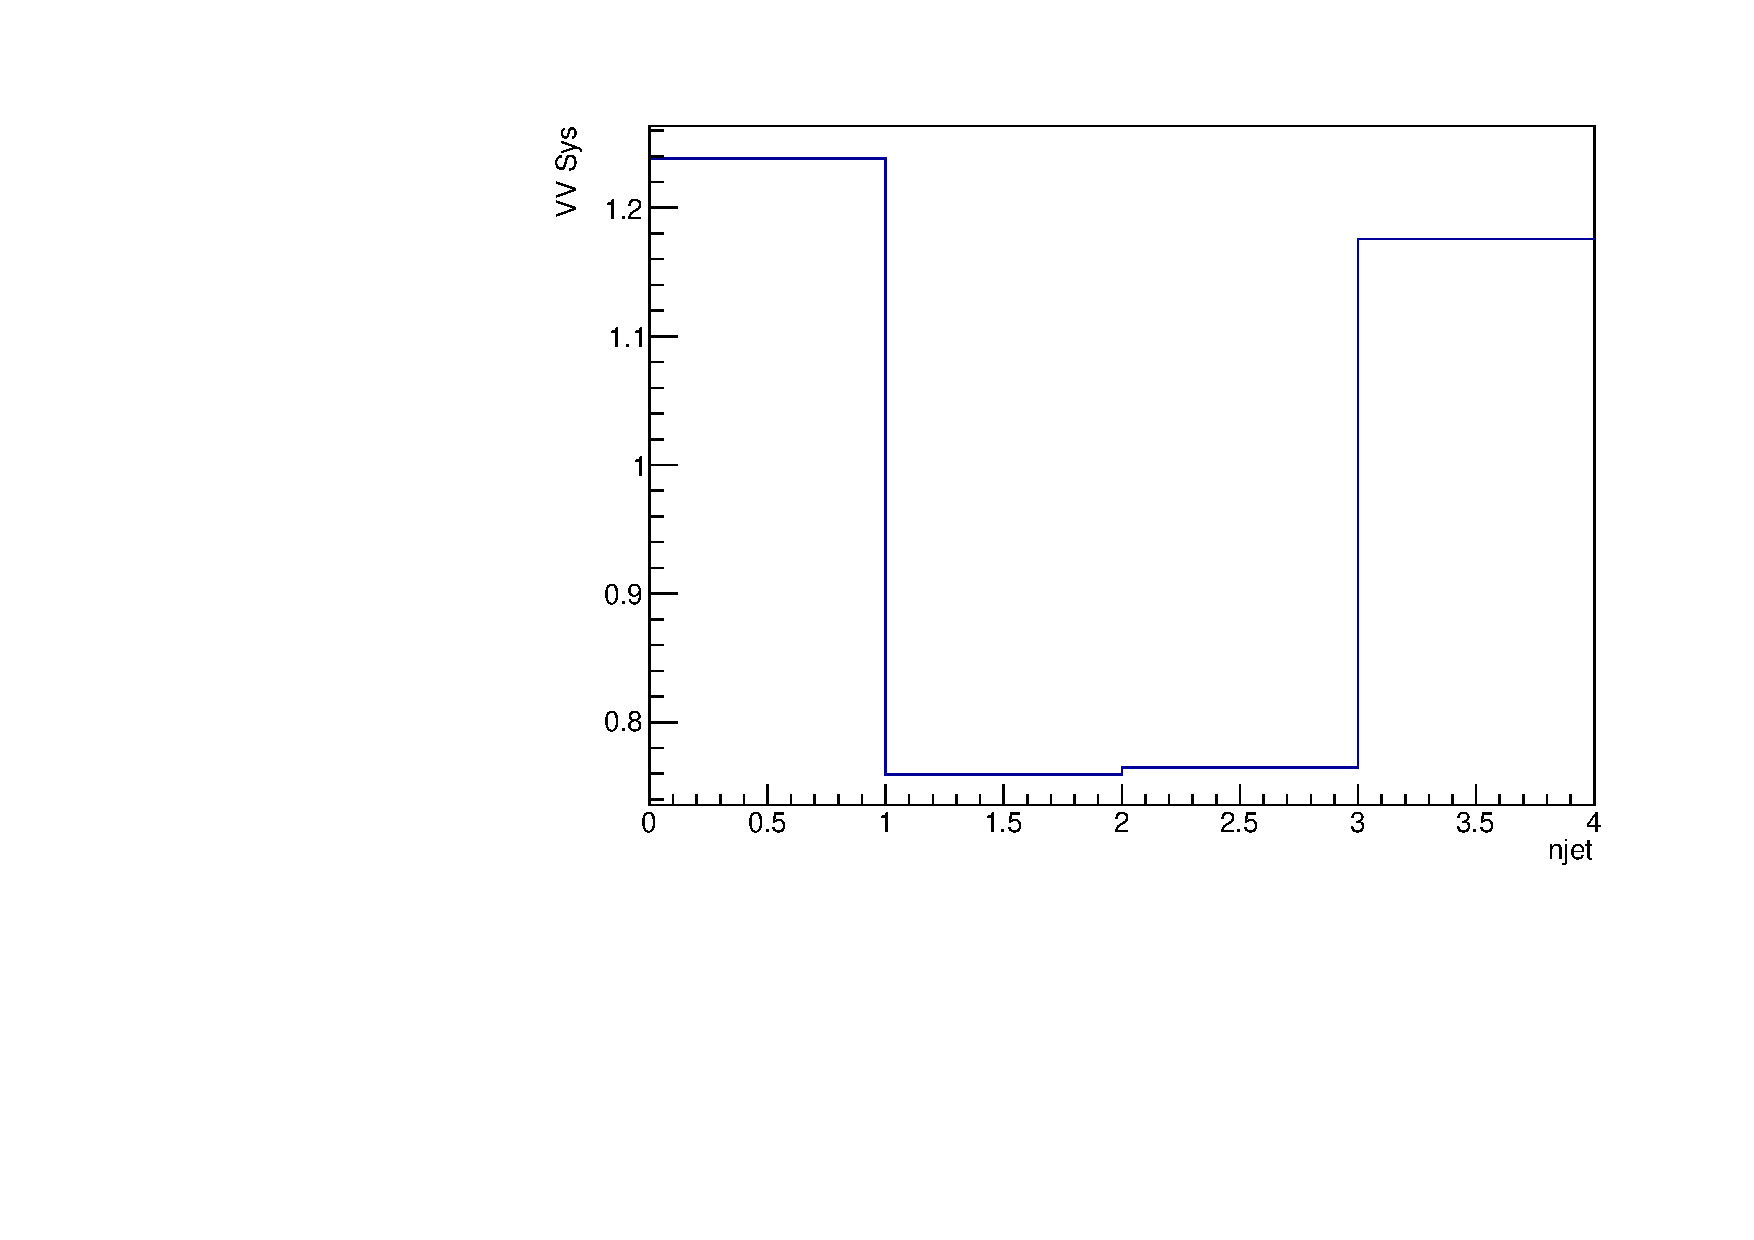
\includegraphics[width=0.325\textwidth]{figures/Part3/Systematics/2018_VV_Sys_1D}\\
 \end{tabular}
 \caption{Scale factors derived from diboson control region, from left to right: 2016, 2017 and 2018 datasets.}
 \label{fig:SF_VV}
 \end{center}
\end{figure}

This uncertainty is about 10-20$\%$, as is shown in Figure \ref{fig:SF_VV}.
%%%%%%%%%%%%%%%%%%%%%%%%%%%%%%%%%%%%%%%%%%%%%%%%%%%%%%%%%%%%%
%%%%%%%%%%%%%%%%%%%%%%%%%%%%%%%%%%%%%%%%%%%%%%%%%%%%%%%%%%%%%
\section{Other Experimental Uncertainties}
\label{sec:OthUnc}

\begin{itemize}
\item Lepton reconstruction, identification, and isolation: electron/muon reconstruction uncertainties are provided by relevant POG. Uncertainties associated with lepton identification and isolation scale factors were evaluated by the authors of the mvaTOP ID cite{mvaTOP}. The statistical components of these uncertainties are treated as uncorrelated while the other components are treated as fully correlated. For high $p_{T}$ muons ($p_{T}>$200GeV), an additional uncertainty (denoted ``muIDHighPt") is assigned and it increases linearly from 0 to 10$\%$ (200GeV-1000GeV) and is caped at $10\%$ after 1000GeV.
\item Muon scale uncertainties: uncertainties on muon momentum (denoted ``MuonScale") are assigned using different method according to the muon $p_{T}$: Rochester algorithm is used for low $p_{T}$ muons ($p_{T}<$200Gev), while GEcite{GEmethod} method is used for high $p_T$ muons ($p_{T}>$200Gev).
\item b-tagging: b-tagging efficiency and uncertainty is provided by the BTV group. 
\item trigger scale factor: trigger scale factors are set to 1 and a flat 2$\%$ uncertainty is assigned. This uncertainty is treated as uncorrelated.
\item Luminosity: The uncertainties of 1.0$\%$, 2.0$\%$ and 1.5$\%$  are assigned to the integrated luminosity for 2016, 2017, 2018, respectively. When processing the run 2 data the individual year uncertainties are treated as uncorrelated while there are two additional correlated luminosity uncertainties; firstly, 0.6$\%$, 0.9$\%$ and 2.0$\%$ for each year respectively to account for the correlation between 2016, 2017 and 2018 data and secondly, 0.6$\%$,0.2$\%$ for 2017 and 2018 respectively to account for the correlation between 2017 and 2018 data. 
\item jet energy scale and resolution: The jet energy scale, JES, and jet energy resolution, JER, are centrally provided by the JET/MET POG cite{JEC}. Variations of jet energy scale and resolution are propagated to the MET and b-tagging SF.
\item pile-up reweighting: The measured minimum bias cross-section is varied up and down by 4.6$\%$. This uncertainty is treated as correlated. 
\item MET unclustered missing energy is considered and treated as uncorrelated across the years.
\item L1 ECAL prefiring: In the 2016 and 2017 datasets, L1 EGamma triggers fired early causing many uninteresting events to be recorded while the later interesting events were rejected. Since this effect is not present in the MC simulation, a tool cite{ECALPre} provided by the L1 DPG is used to reweight MC events. This uncertainty is treated as correlated. 
\item HEM15/16 Issue: The HEM15/16 issue refers to two HCAL modules whose power supply died in 
the middle of the data taking (runs$>=$319077, i.e. last certified run of 
2018B, and all of 2018C+D). The HEM issue is likely a very small effect but we still have to check it following the procedure in cite{HEM}
\end{itemize}

Uncertainties related to B-tagging scale factors are split into different sources. For b and udsg jets, we applied lf, hf, hfstats1/2, and lfstats1/2 uncertainties. For c jets, we applied cferr1/2 uncertainties. Correlations between different sources are specified in the Table~\ref{tab:btag}.

\begin{table}[!hbtp]
\label{tab:btag}
\sffamily
\begin{center}
\caption{
A hyphen ($-$) denotes that a source is not correlated between the different years.
}
\begin{tabular}{|l|c|l|}
\hline
Source & Correlated & Description\\
\hline
lf			& \checkmark & udsg+c jets in heavy flavor region\\ %HF$^1$
hf			& \checkmark & b+c jets in light flavor region \\ %LF$^2$
hfstats1	& - 		 & Linear fluctuations of c jets\\
hfstats2	& -			 & Quadratic fluctuations of c jets \\
lfstats1	& -			 & Linear fluctuations of udsg jets \\
lfstats2	& -			 & Quadratic fluctuations of udsg jets \\
cferr1		& \checkmark & Linear fluctuations of c jets \\
cferr2		& \checkmark & Quadratic fluctuations of c jets \\
\hline
\end{tabular}
\end{center}
\end{table}

\subsection{Jet energy scale uncertainties}

Uncertainties associated with JES are split into their 27 components and properly treated the correlations of the split uncertainties by year as recommended by the JETMET POG and described in the Table \ref{tab:jec}.

\begin{table}[!hbtp]
\sffamily
\begin{center}
\caption{
Summary of the sources of uncertainty related to the JECs.
A hyphen ($-$) denotes that a source is not correlated between the different years.
}
\label{tab:jec}
\begin{tabular}{|l|c|}
\hline
Source & Correlated\\
\hline
AbsoluteStat			& -			 \\
AbsoluteScale			& \checkmark			 \\
AbsoluteMPFBias			& \checkmark 		 	 \\
Fragmentation			& \checkmark			 \\
SinglePionECAL			& \checkmark			 \\
SinglePionHCAL			& \checkmark			 \\
FlavorQCD				& \checkmark			 \\
TimePtEta				& -			 \\
RelativeJEREC1			& -			 \\
RelativeJEREC2			& -			 \\
RelativeJERHF			& \checkmark			 \\
RelativePtBB			& \checkmark			 \\
RelativePtEC1			& -			 \\
RelativePtEC2			& -			 \\
RelativePtHF			& \checkmark			 \\
RelativeBal				& \checkmark			 \\
RelativeSample			& -			 \\
RelativeFSR				& -			 \\
RelativeStatFSR			& \checkmark			 \\
RelativeStatEC			& -			 \\
RelativeStatHF			& -			 \\
PileUpDataMC			& \checkmark			 \\
PileUpPtRef				& \checkmark			 \\
PileUpPtBB				& \checkmark			 \\
PileUpPtEC1				& \checkmark			 \\
PileUpPtEC2				& \checkmark			 \\
PileUpPtHF				& \checkmark			 \\
\hline
\end{tabular}
\end{center}
\end{table}

B-tagging scale factors and MET vector are computed for each of the JES templates and treated as uncertainties that are fully correlated to the respective JES sources. 

The overall systematic uncertainty on background is estimated to be about 15 $\%$ in SR.

 A comparison of different sources of systematic uncertainties of the background estimates in SR is shown in Figure \ref{fig:Comp_sys_background}.

\begin{figure}[tbh!]
 \begin{center}
 \begin{tabular}{cc}
  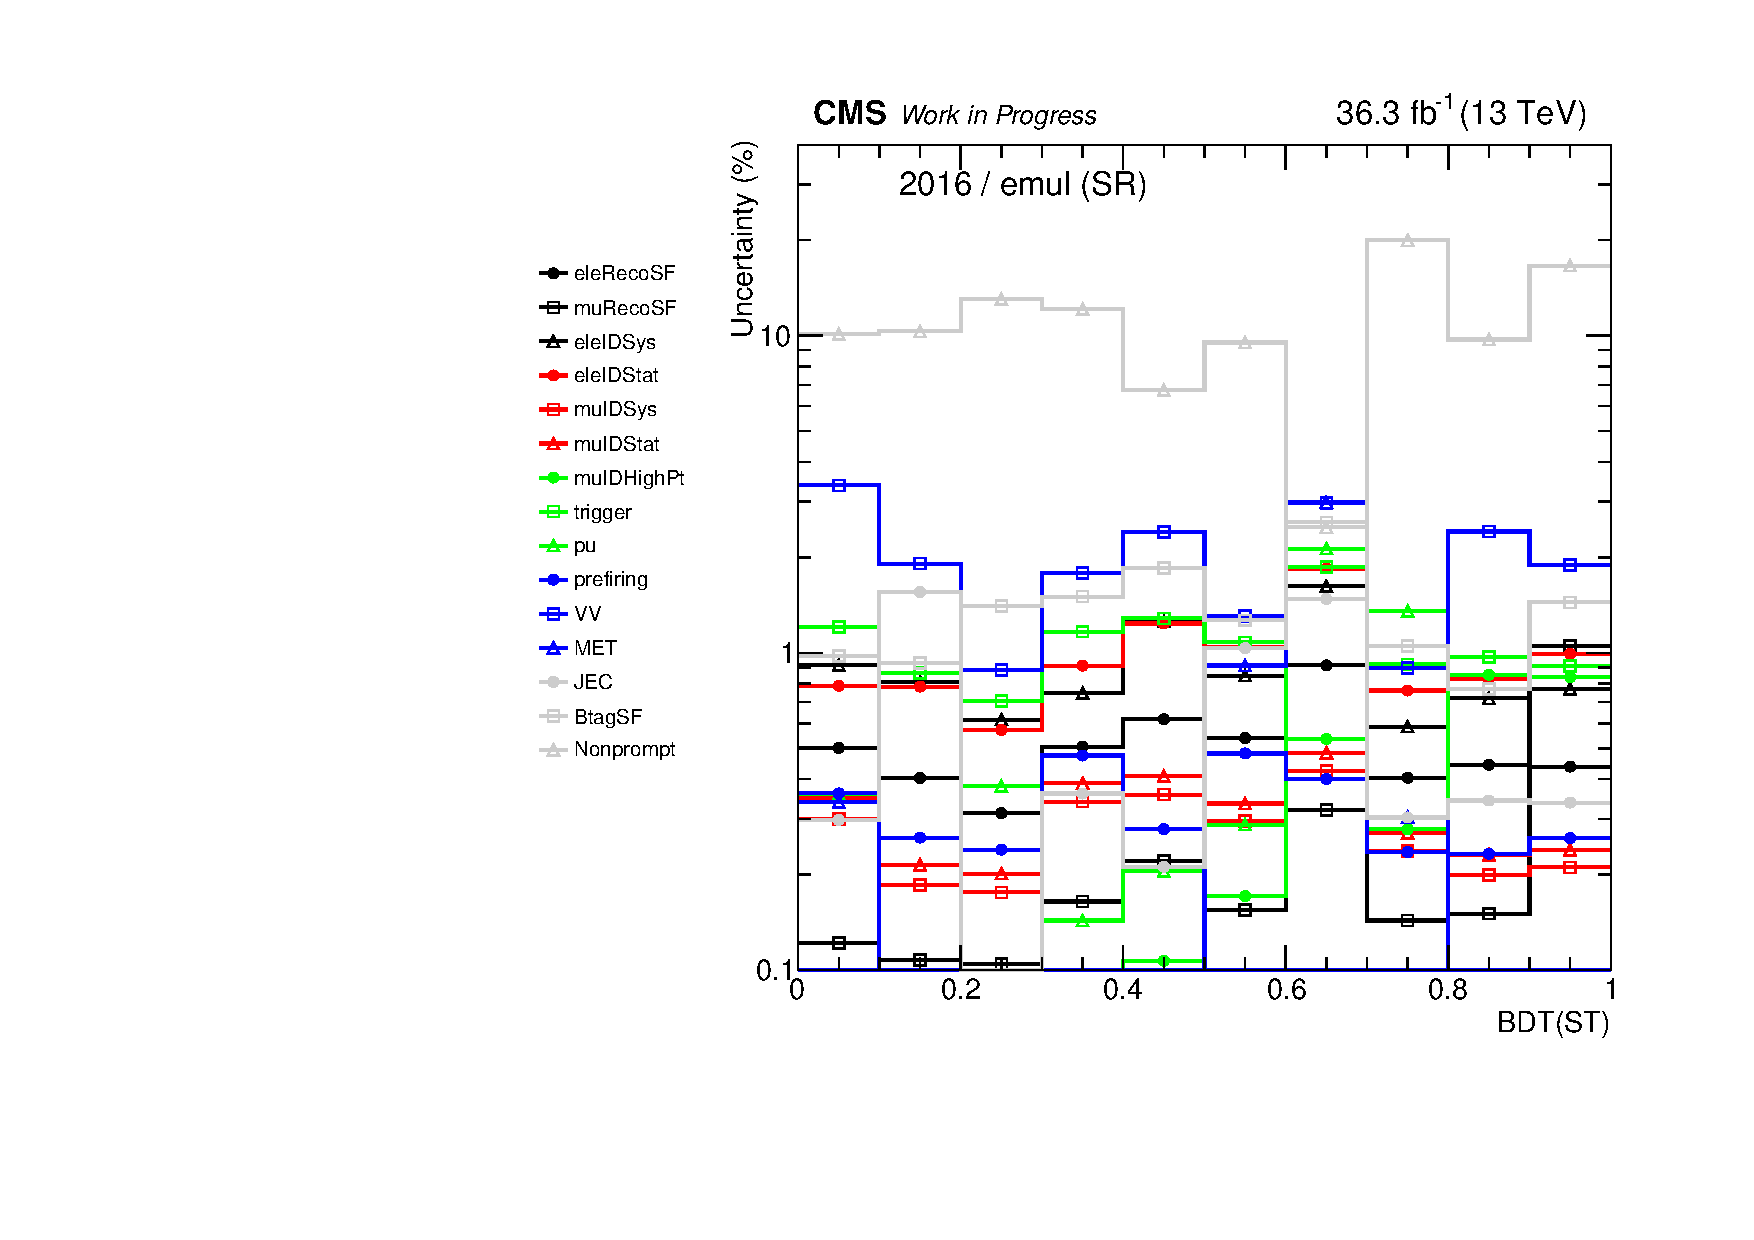
\includegraphics[width=0.45\textwidth]{figures/Part3/Systematics/sysBDT_ST_bkg_2016}&
  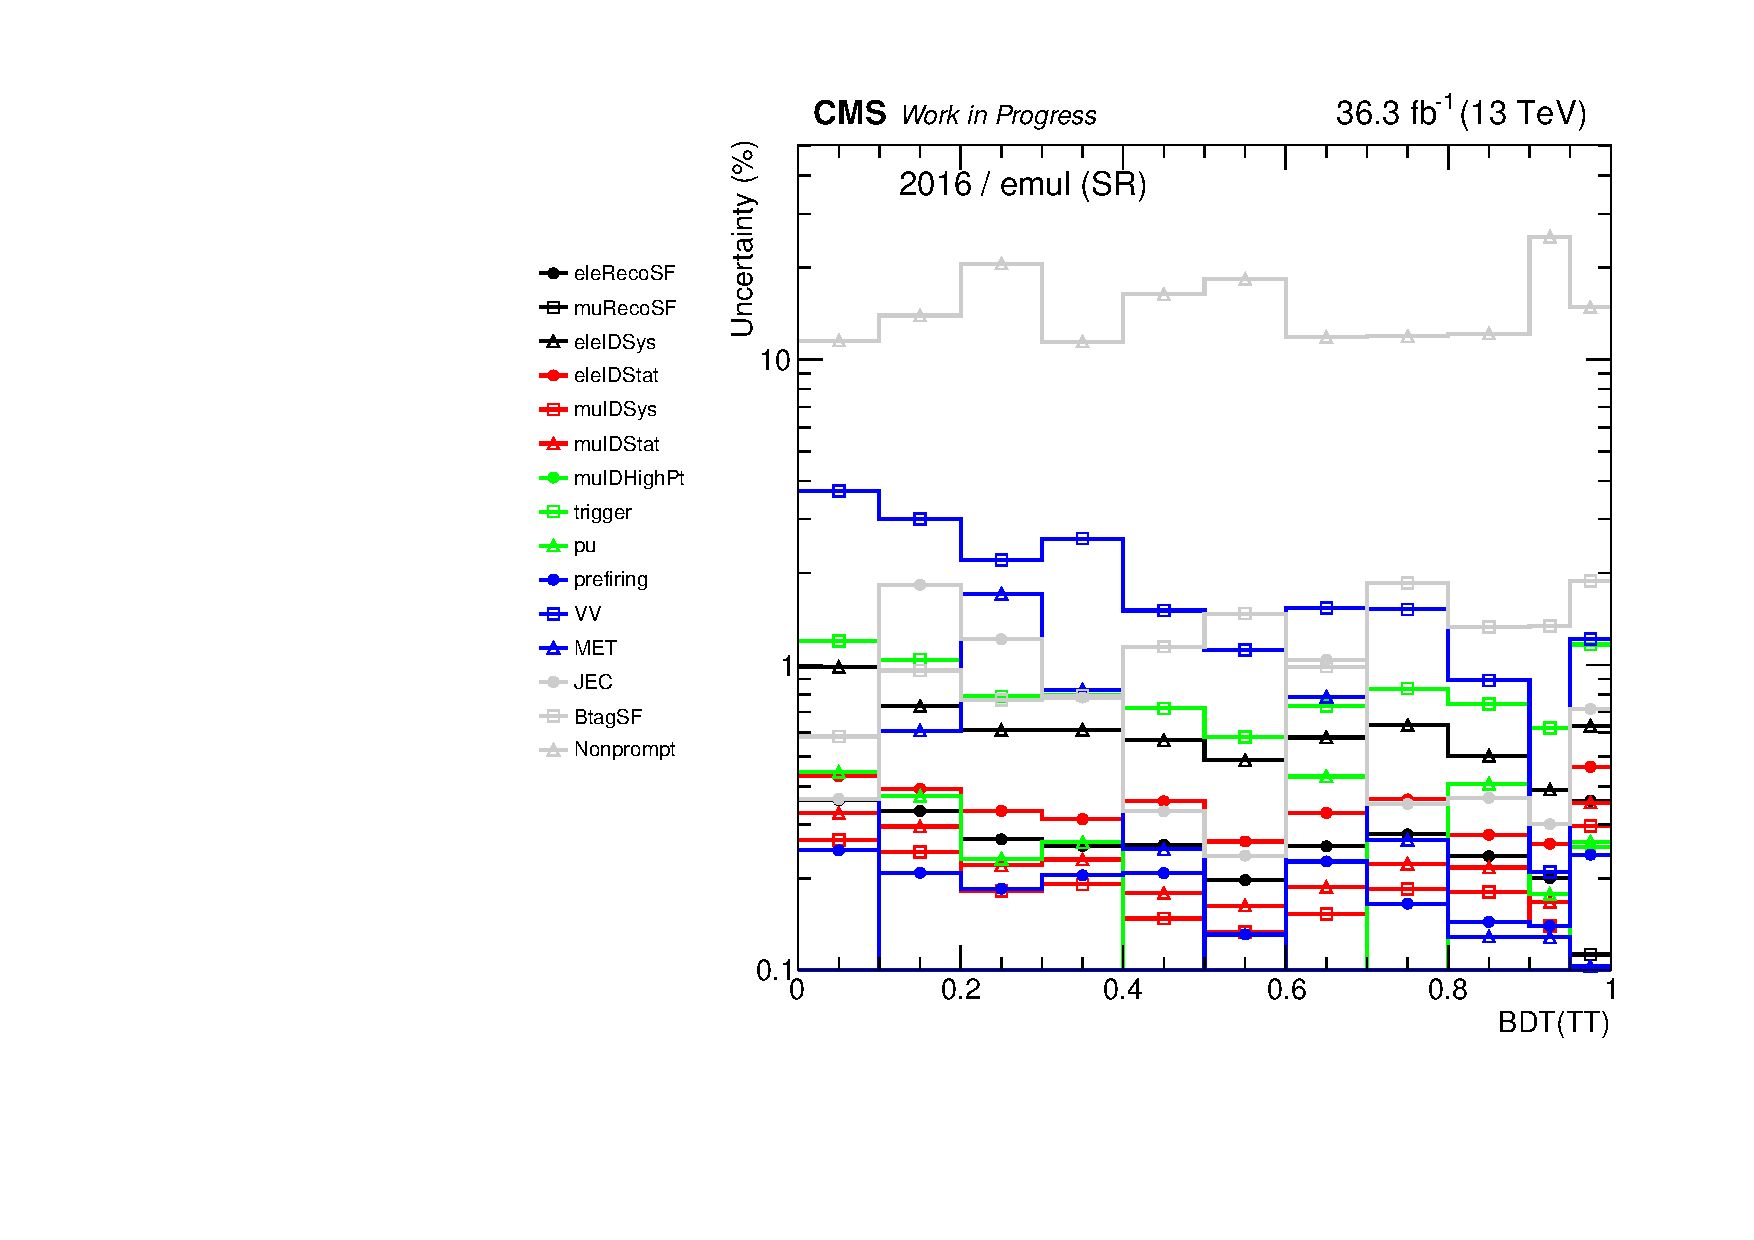
\includegraphics[width=0.45\textwidth]{figures/Part3/Systematics/sysBDT_TT_bkg_2016} \\
    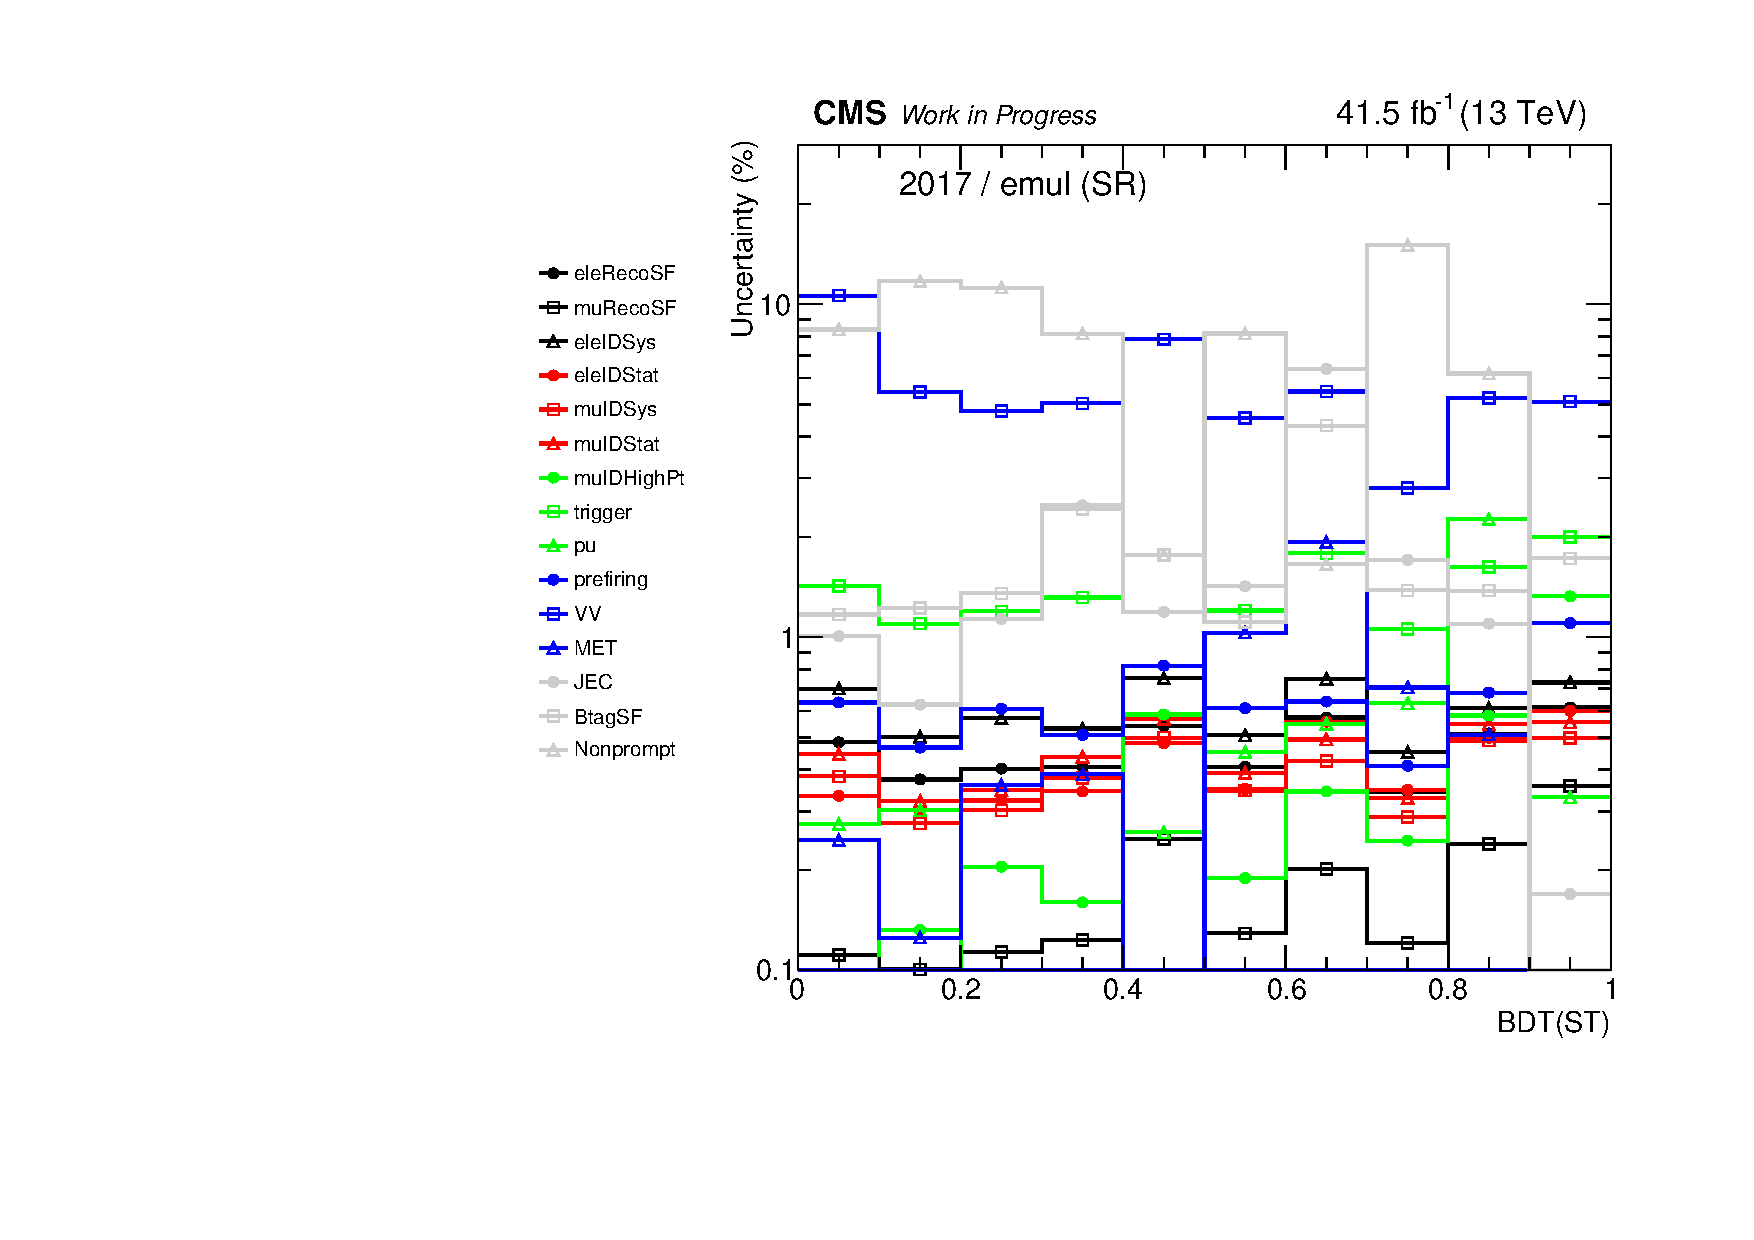
\includegraphics[width=0.45\textwidth]{figures/Part3/Systematics/sysBDT_ST_bkg_2017}&
  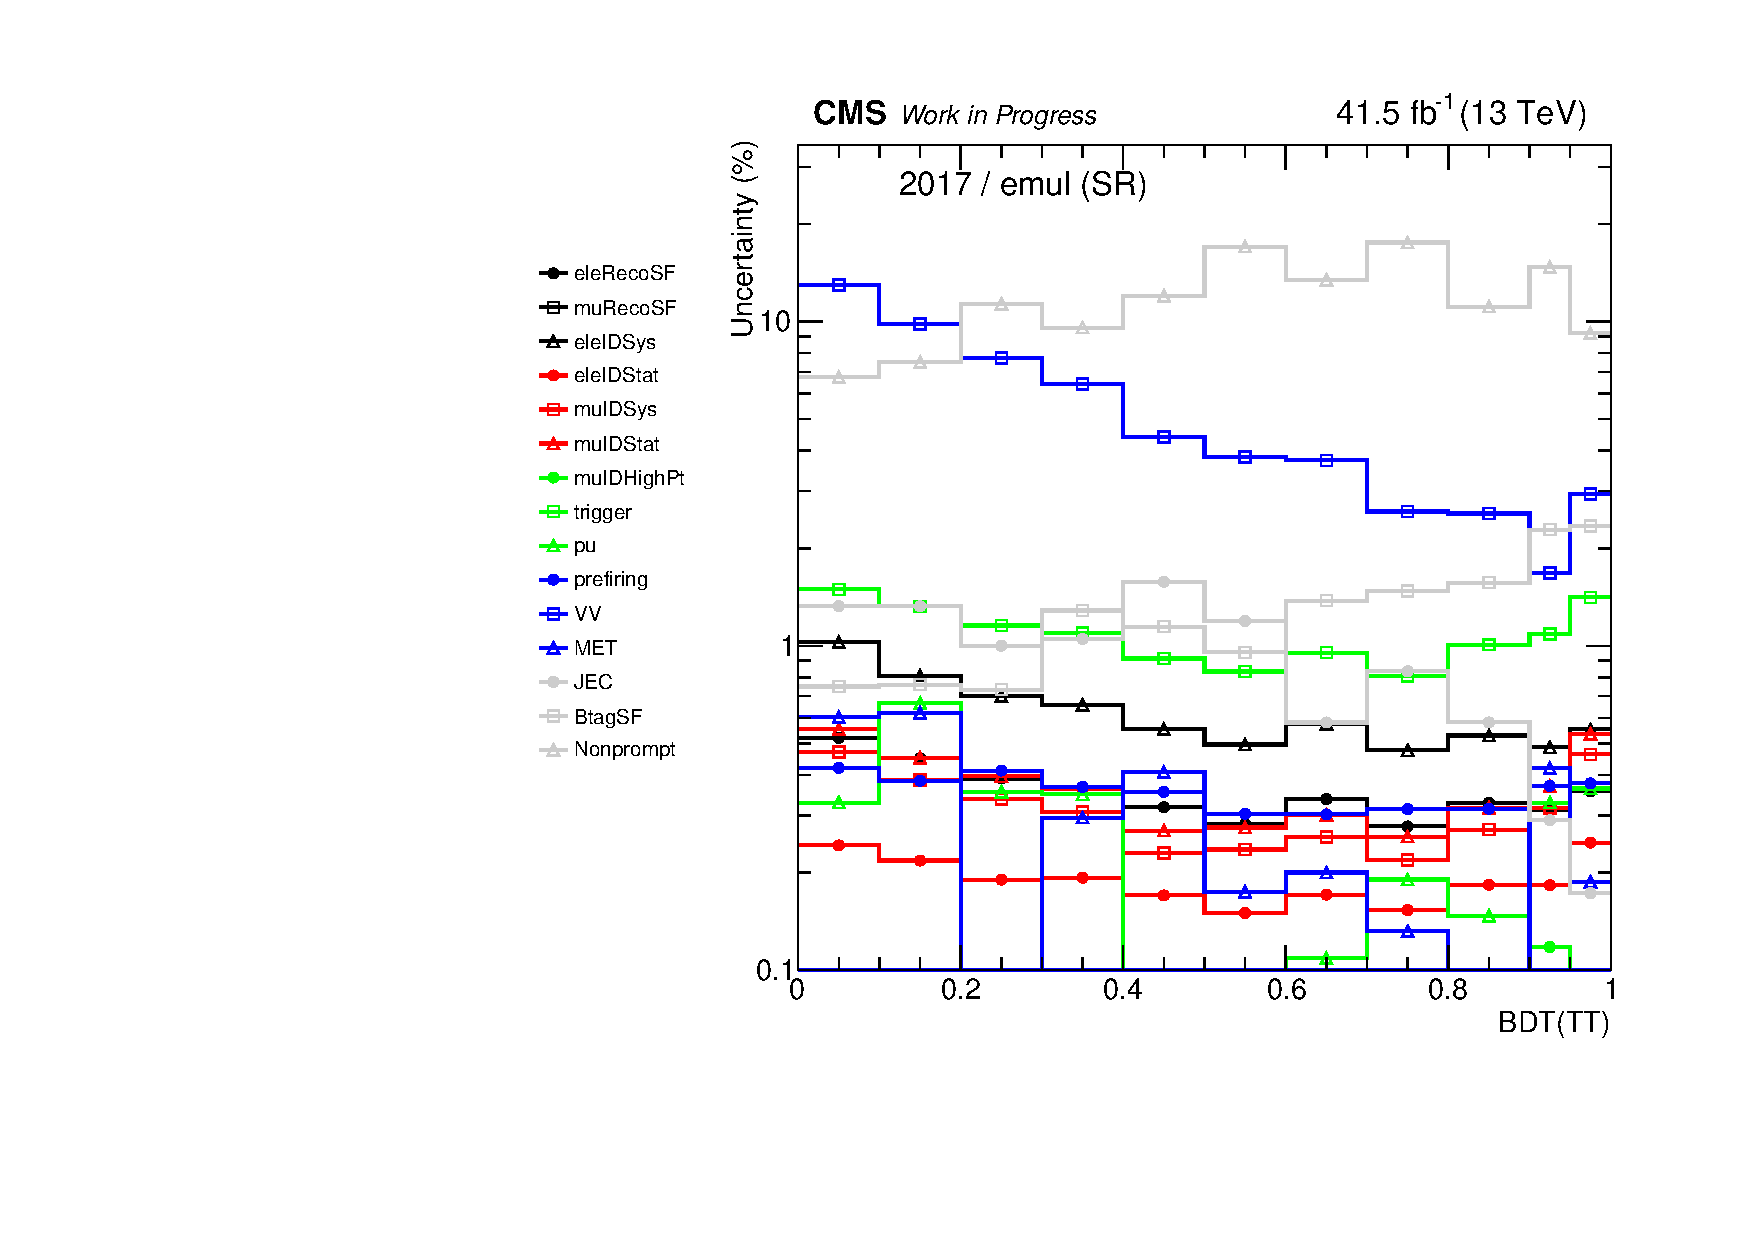
\includegraphics[width=0.45\textwidth]{figures/Part3/Systematics/sysBDT_TT_bkg_2017} \\
    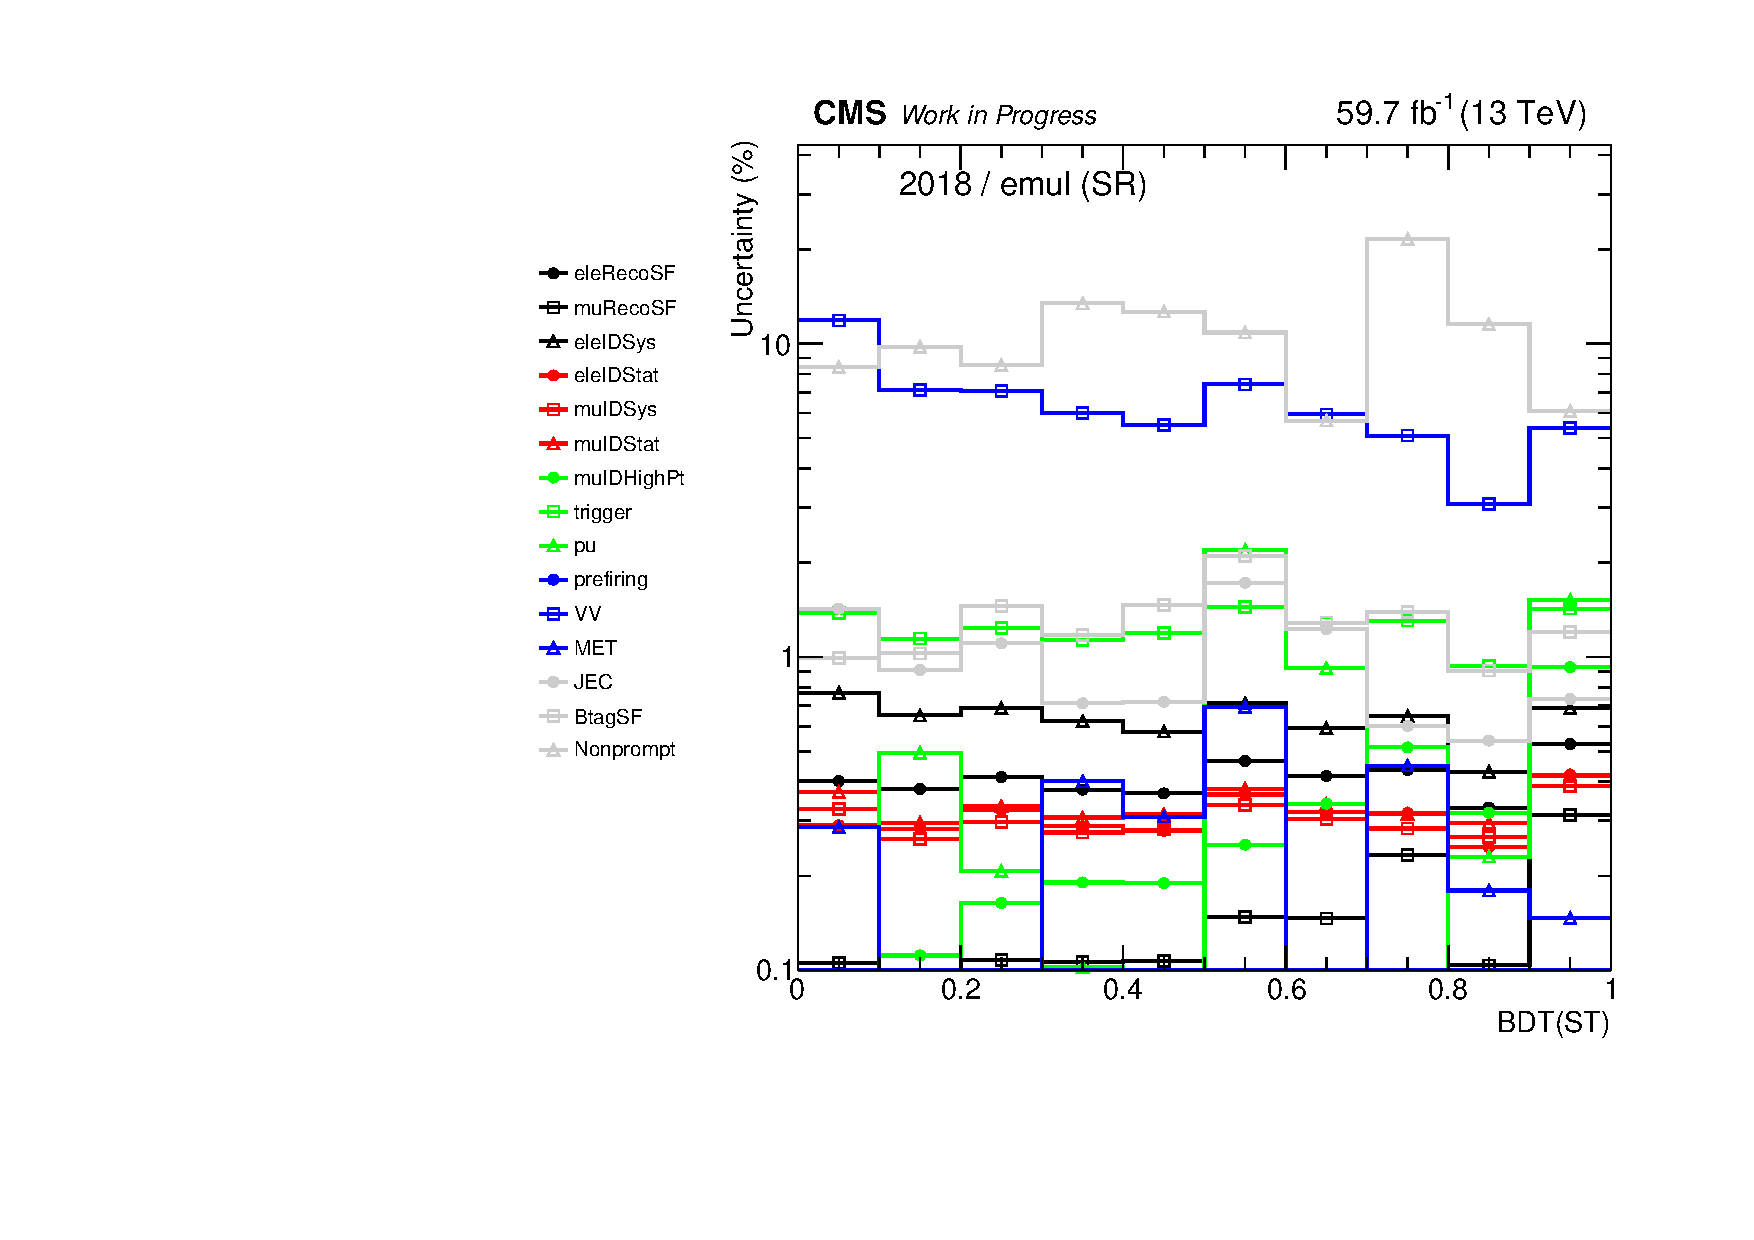
\includegraphics[width=0.45\textwidth]{figures/Part3/Systematics/sysBDT_ST_bkg_2018}&
  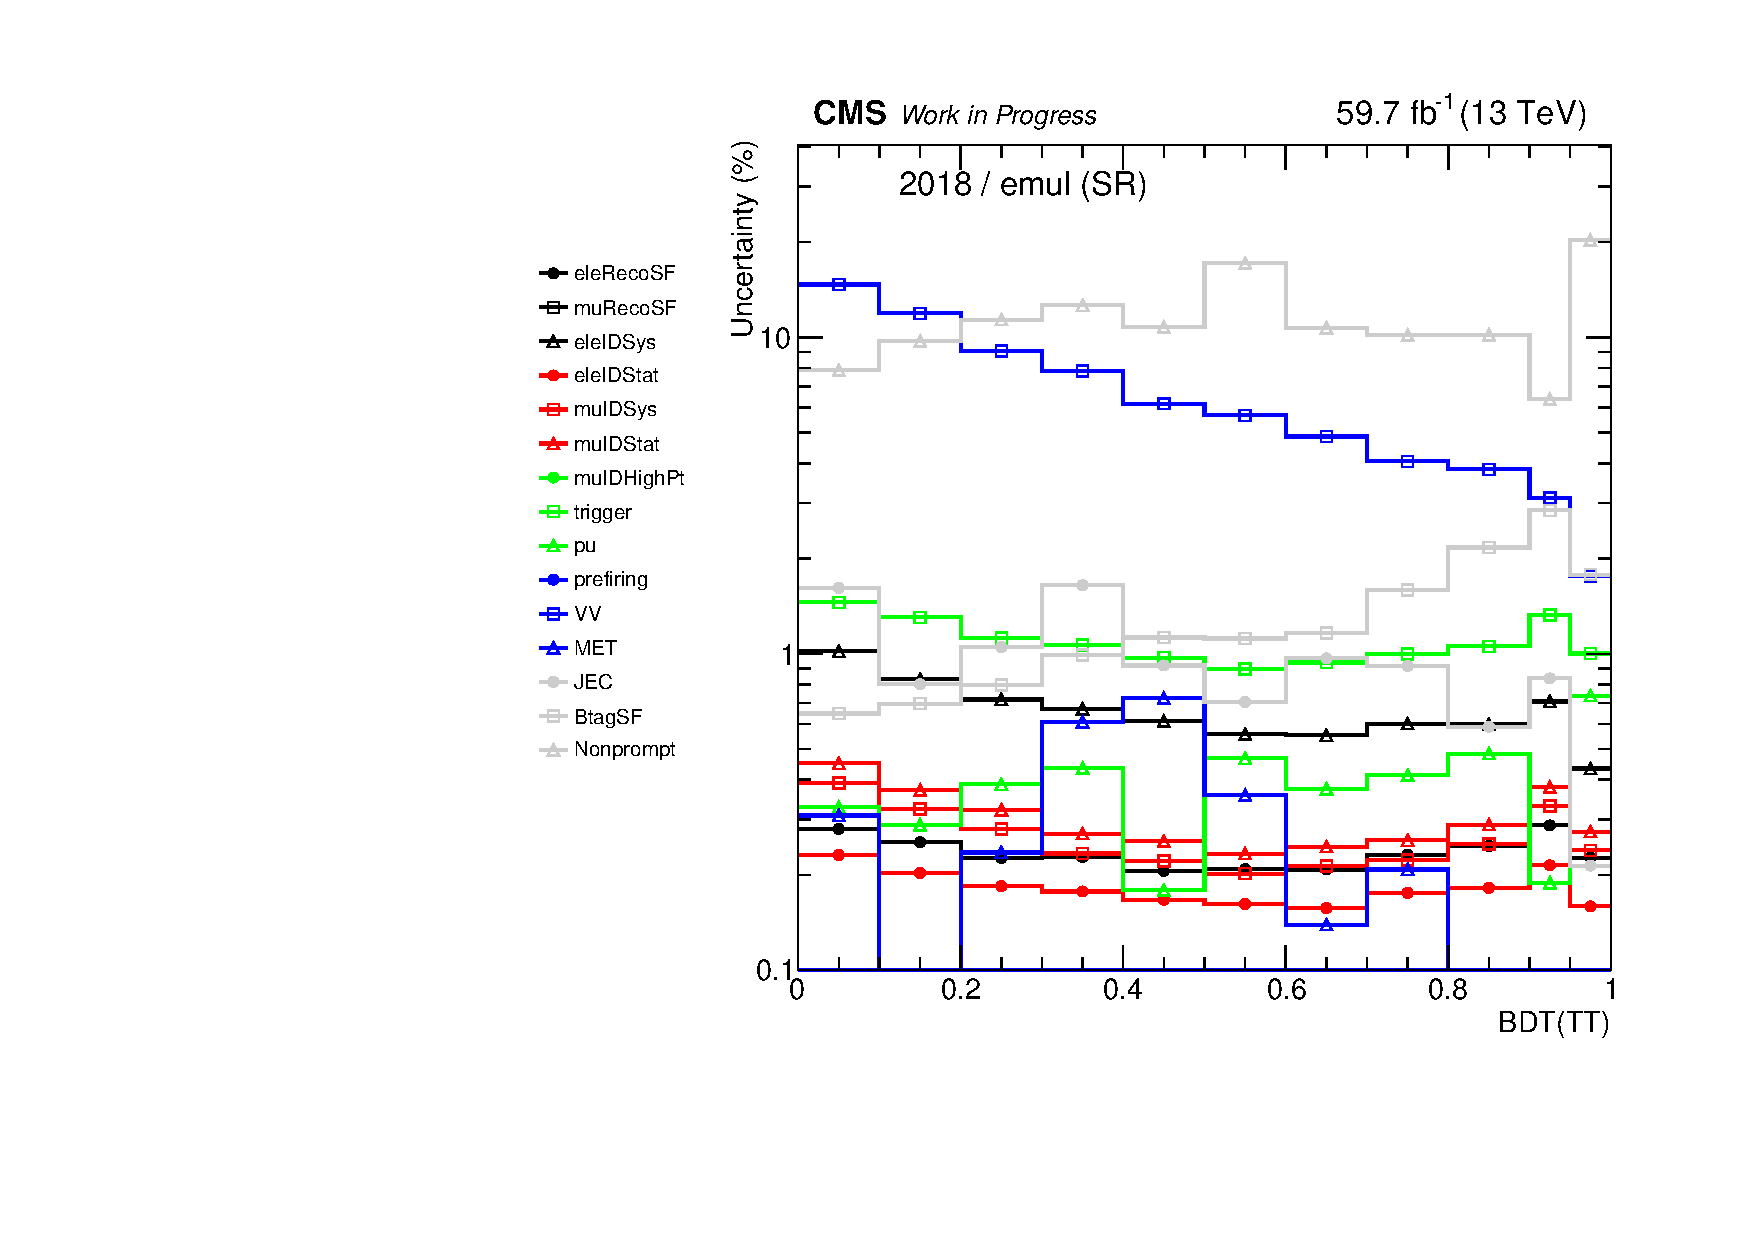
\includegraphics[width=0.45\textwidth]{figures/Part3/Systematics/sysBDT_TT_bkg_2018} \\
 \end{tabular}
 \caption{Distributions of relative uncertainties on total expected backgrounds as a function of BDT output in ST enriched SR (left), TT enriched SR (right). Luminosity and normalization uncertainties are not included in these plots. JES, JER and HEM are combined into "JEC". Sources of b-tagging uncertainties listed in Table~\ref{tab:btag} are combined into "BtagSF". From top to bottom: 2016, 2017 and 2018 datasets.}
 \label{fig:Comp_sys_background}
 \end{center}
\end{figure}

 A comparison of different sources of systematic uncertainties of the signal estimates in SR is shown in Figure \ref{fig:Comp_sys_signal}.

\begin{figure}[tbh!]
 \begin{center}
 \begin{tabular}{cc}
  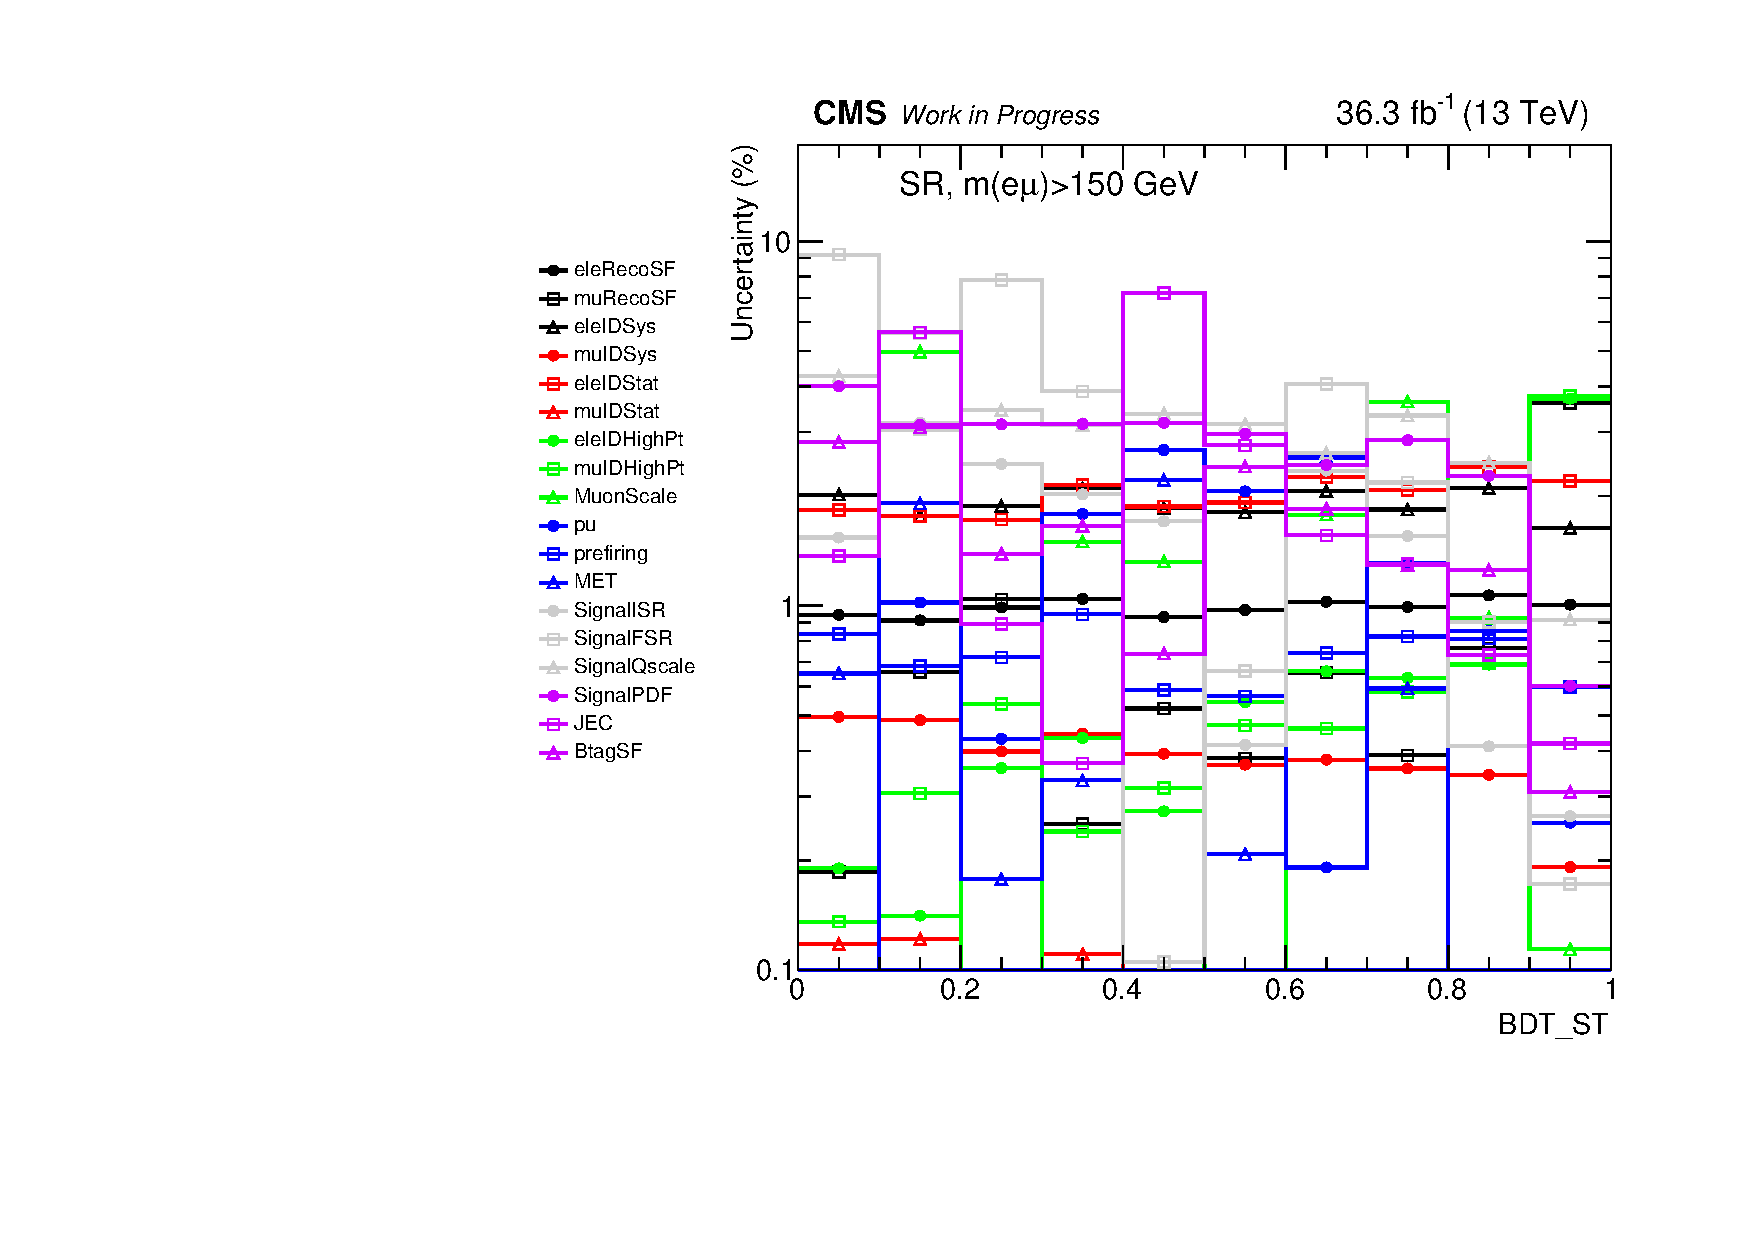
\includegraphics[width=0.45\textwidth]{figures/Part3/Systematics/sysBDT_ST_sig_2016}&
  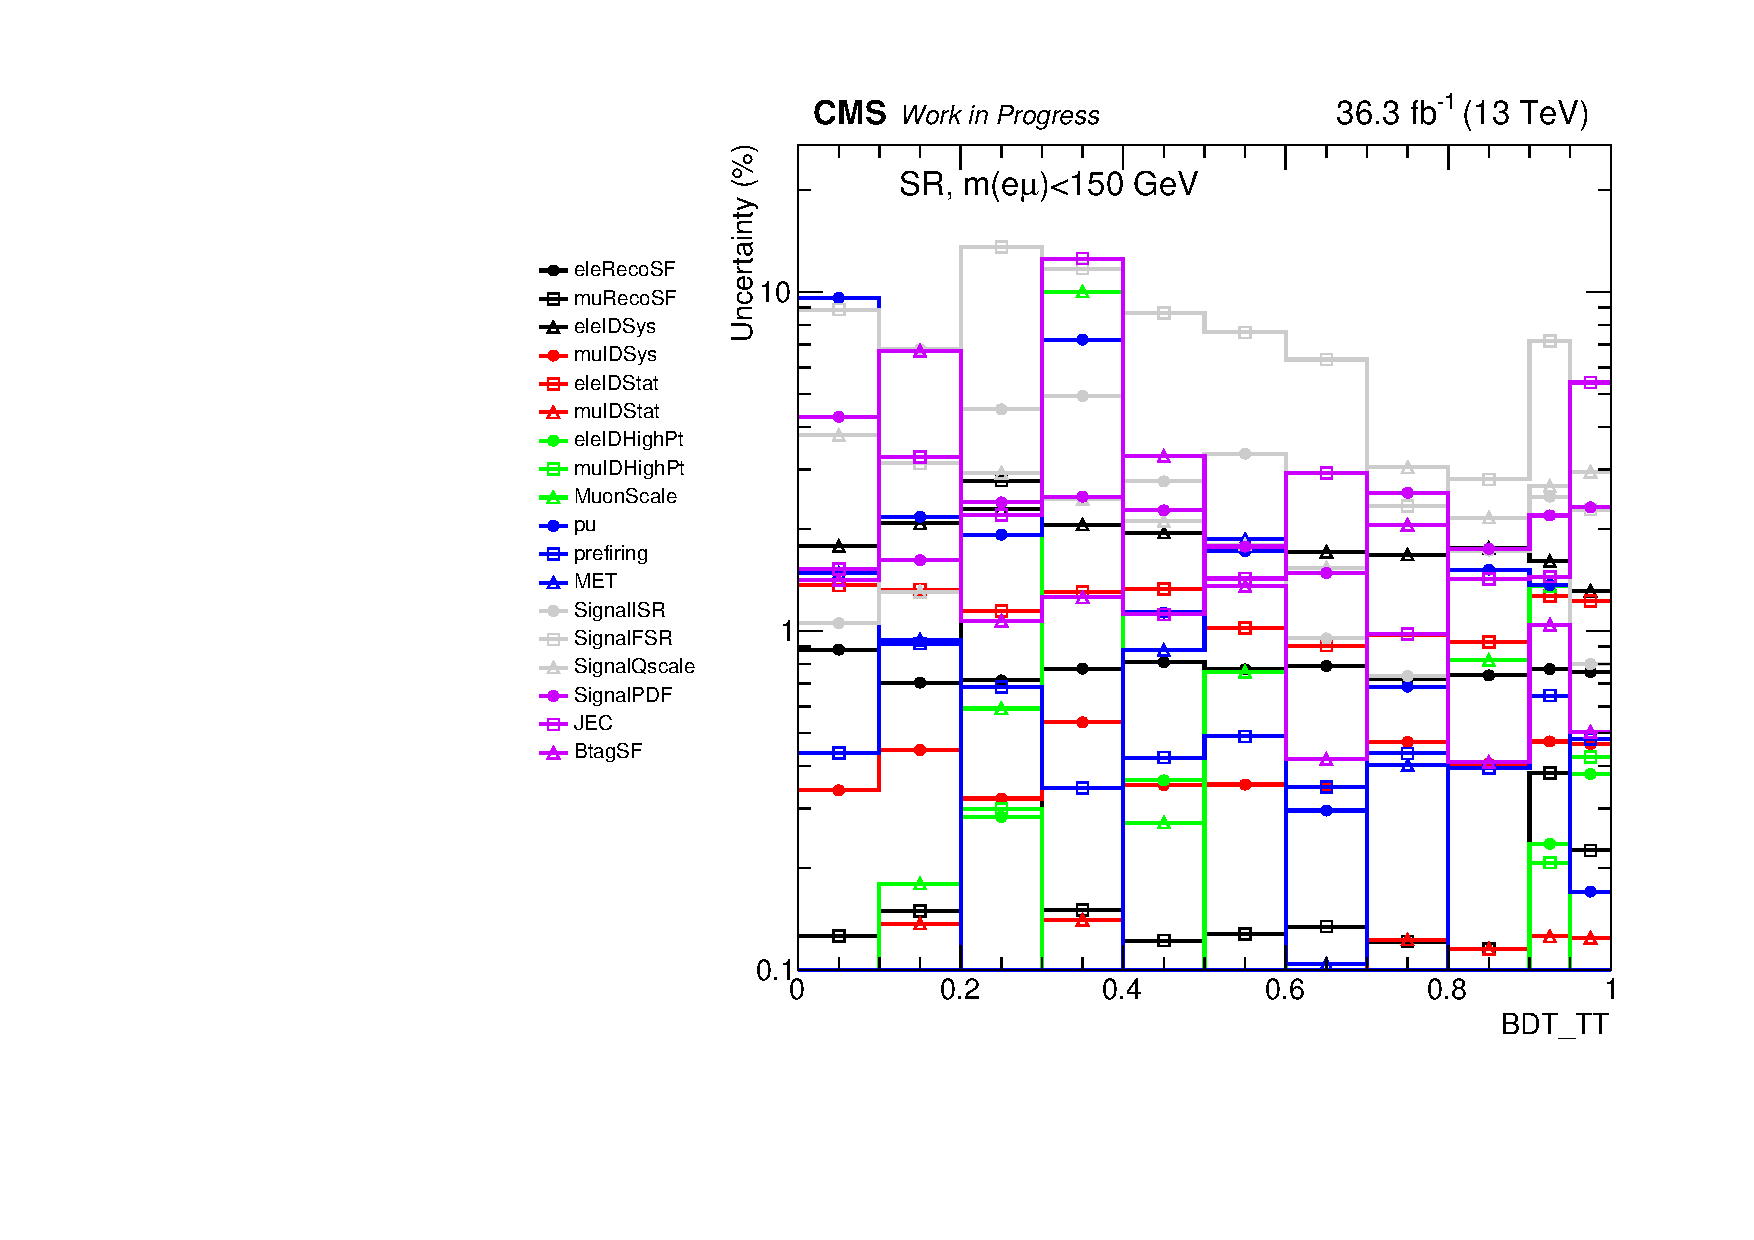
\includegraphics[width=0.45\textwidth]{figures/Part3/Systematics/sysBDT_TT_sig_2016} \\
    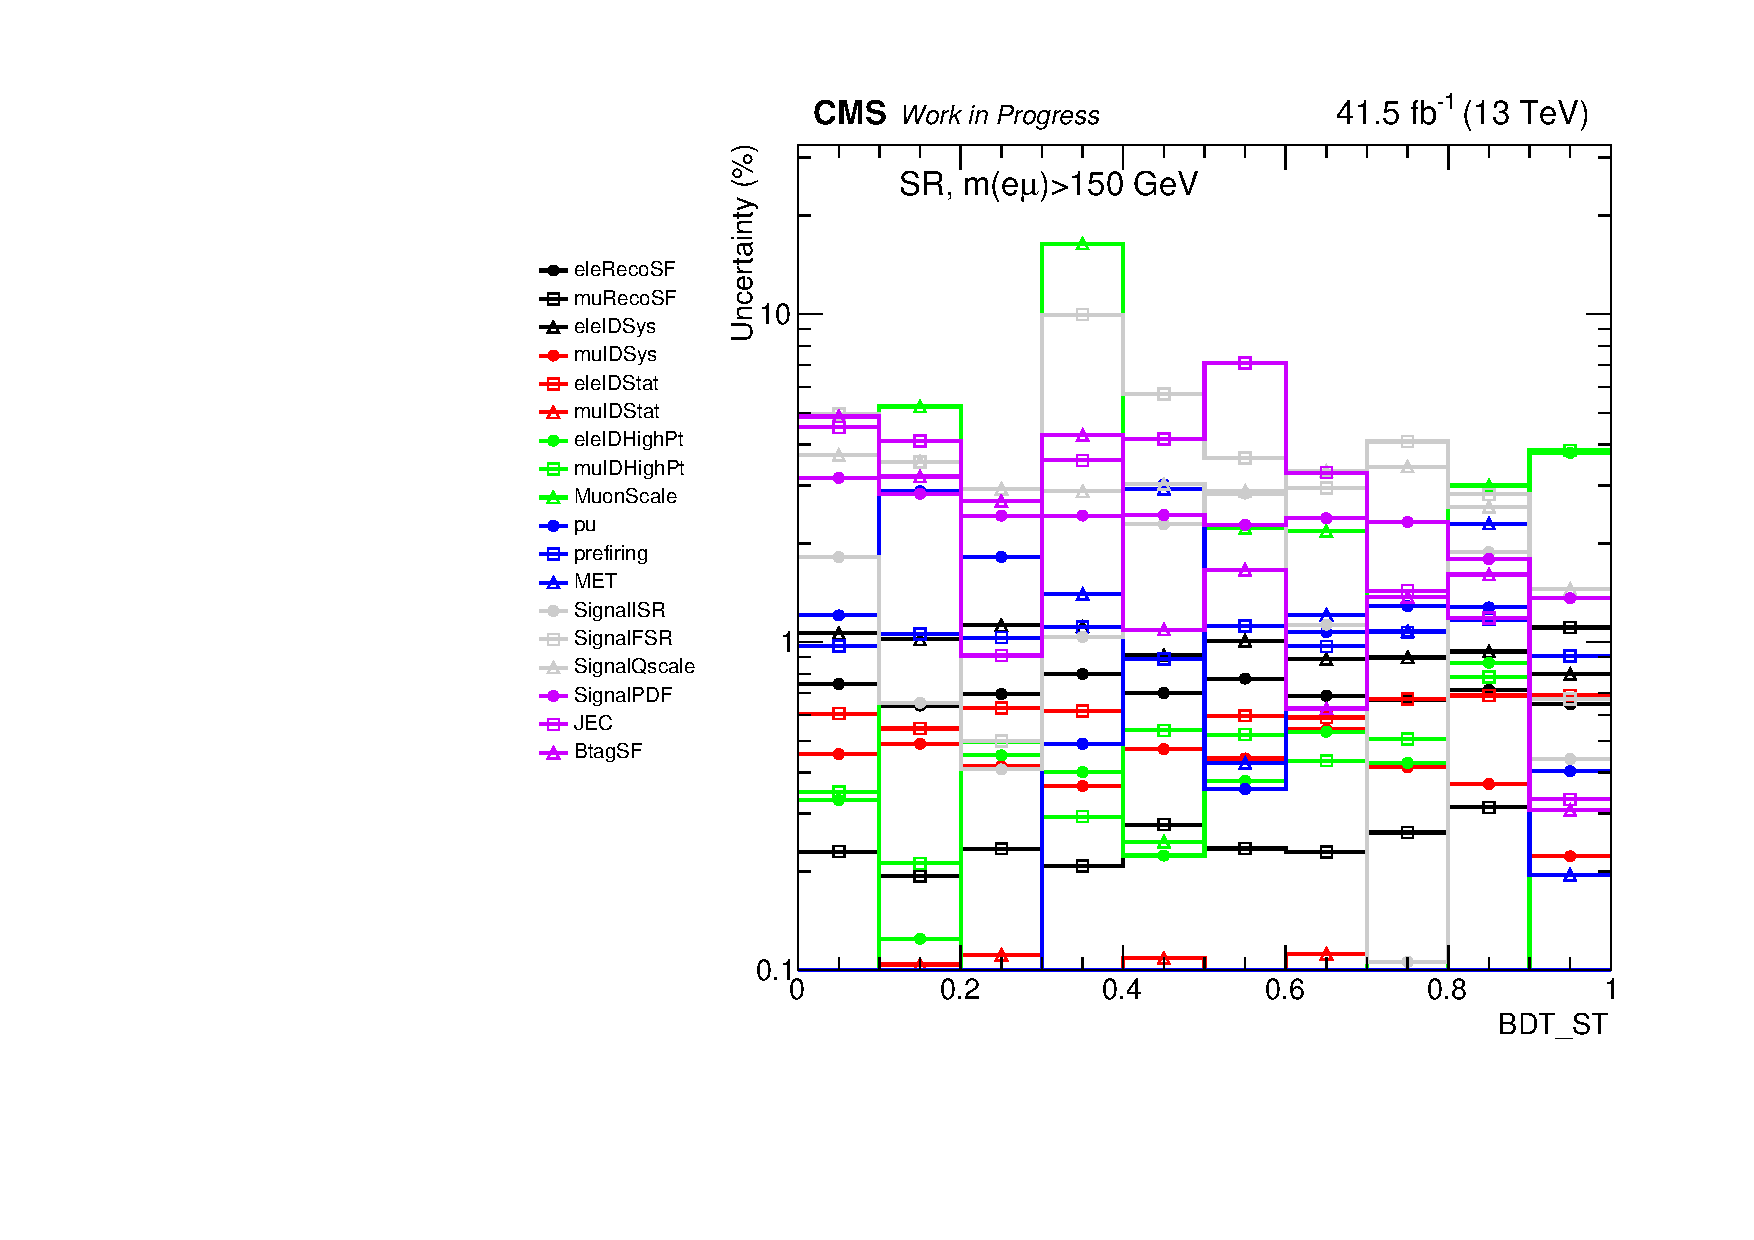
\includegraphics[width=0.45\textwidth]{figures/Part3/Systematics/sysBDT_ST_sig_2017}&
  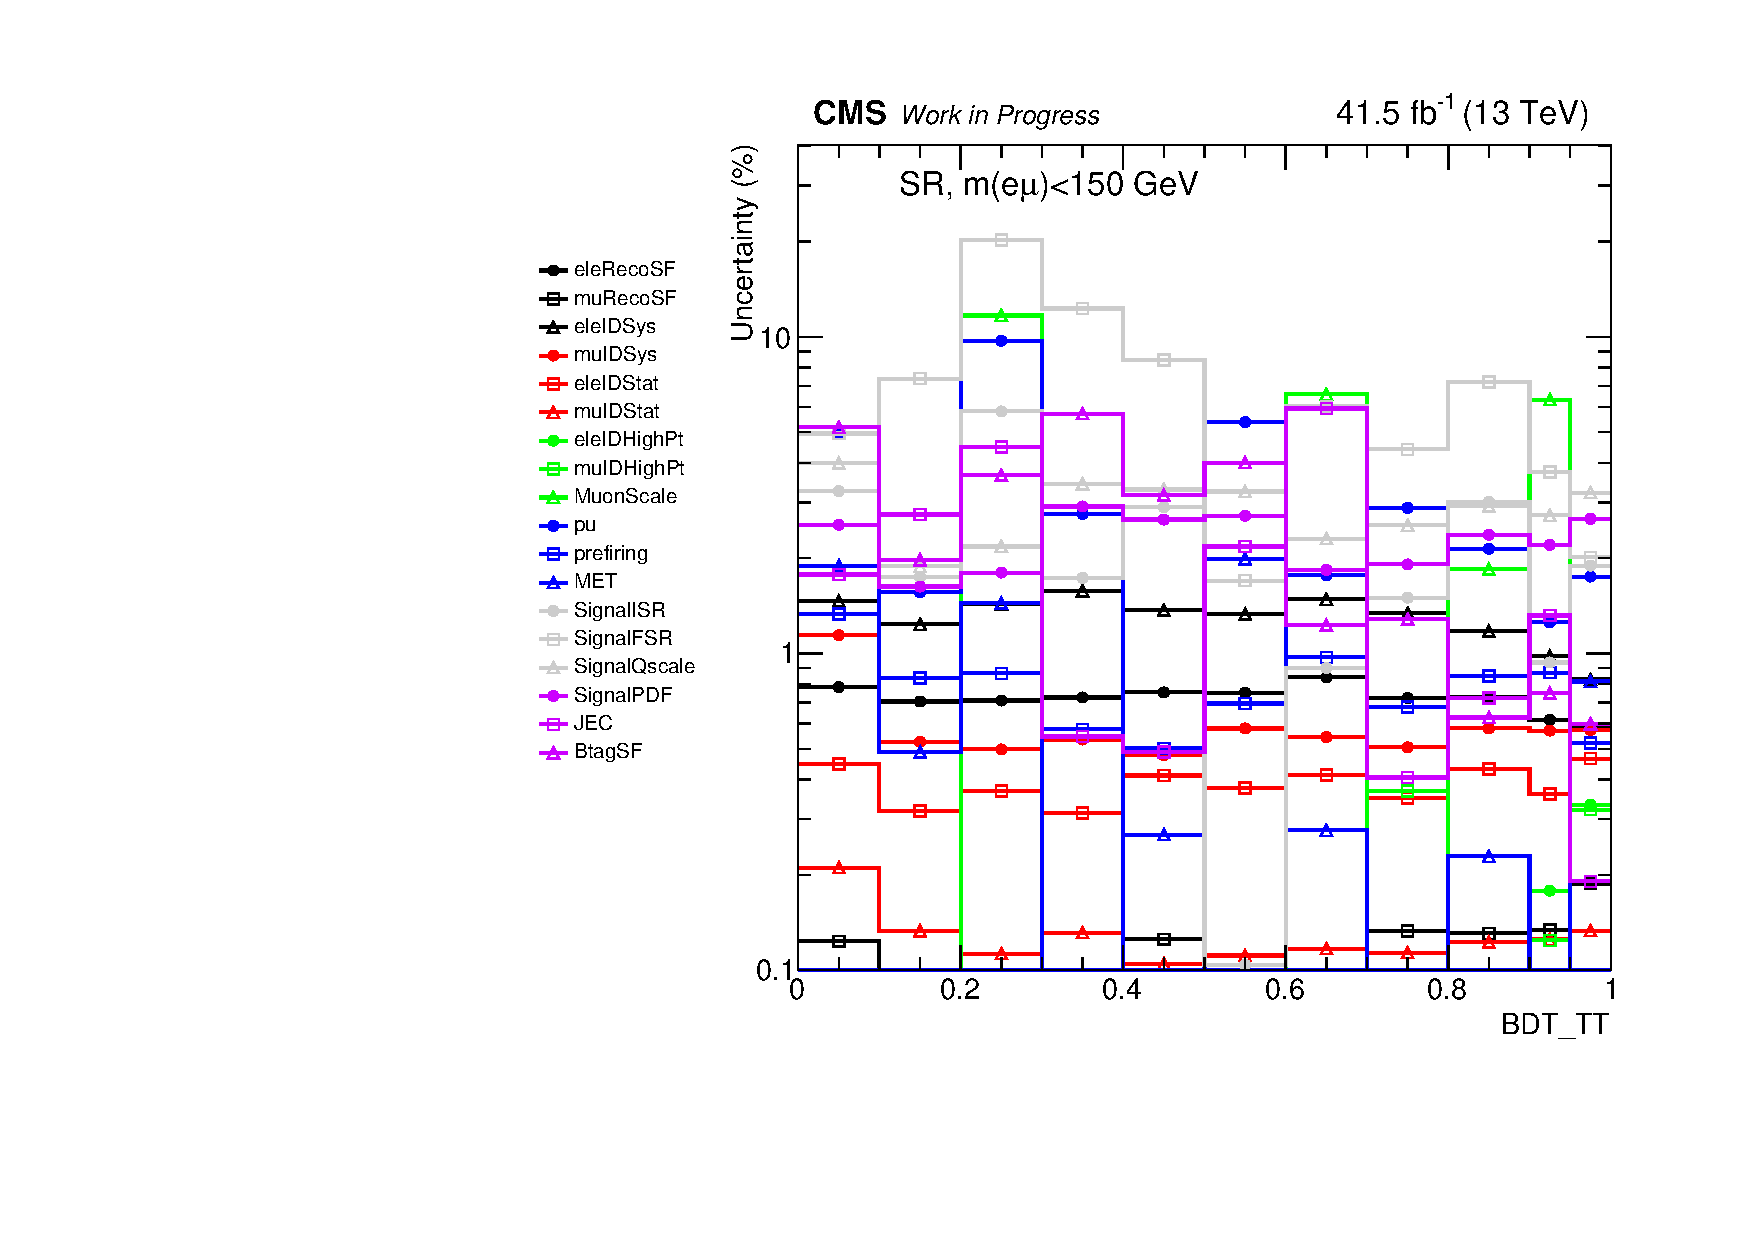
\includegraphics[width=0.45\textwidth]{figures/Part3/Systematics/sysBDT_TT_sig_2017} \\
    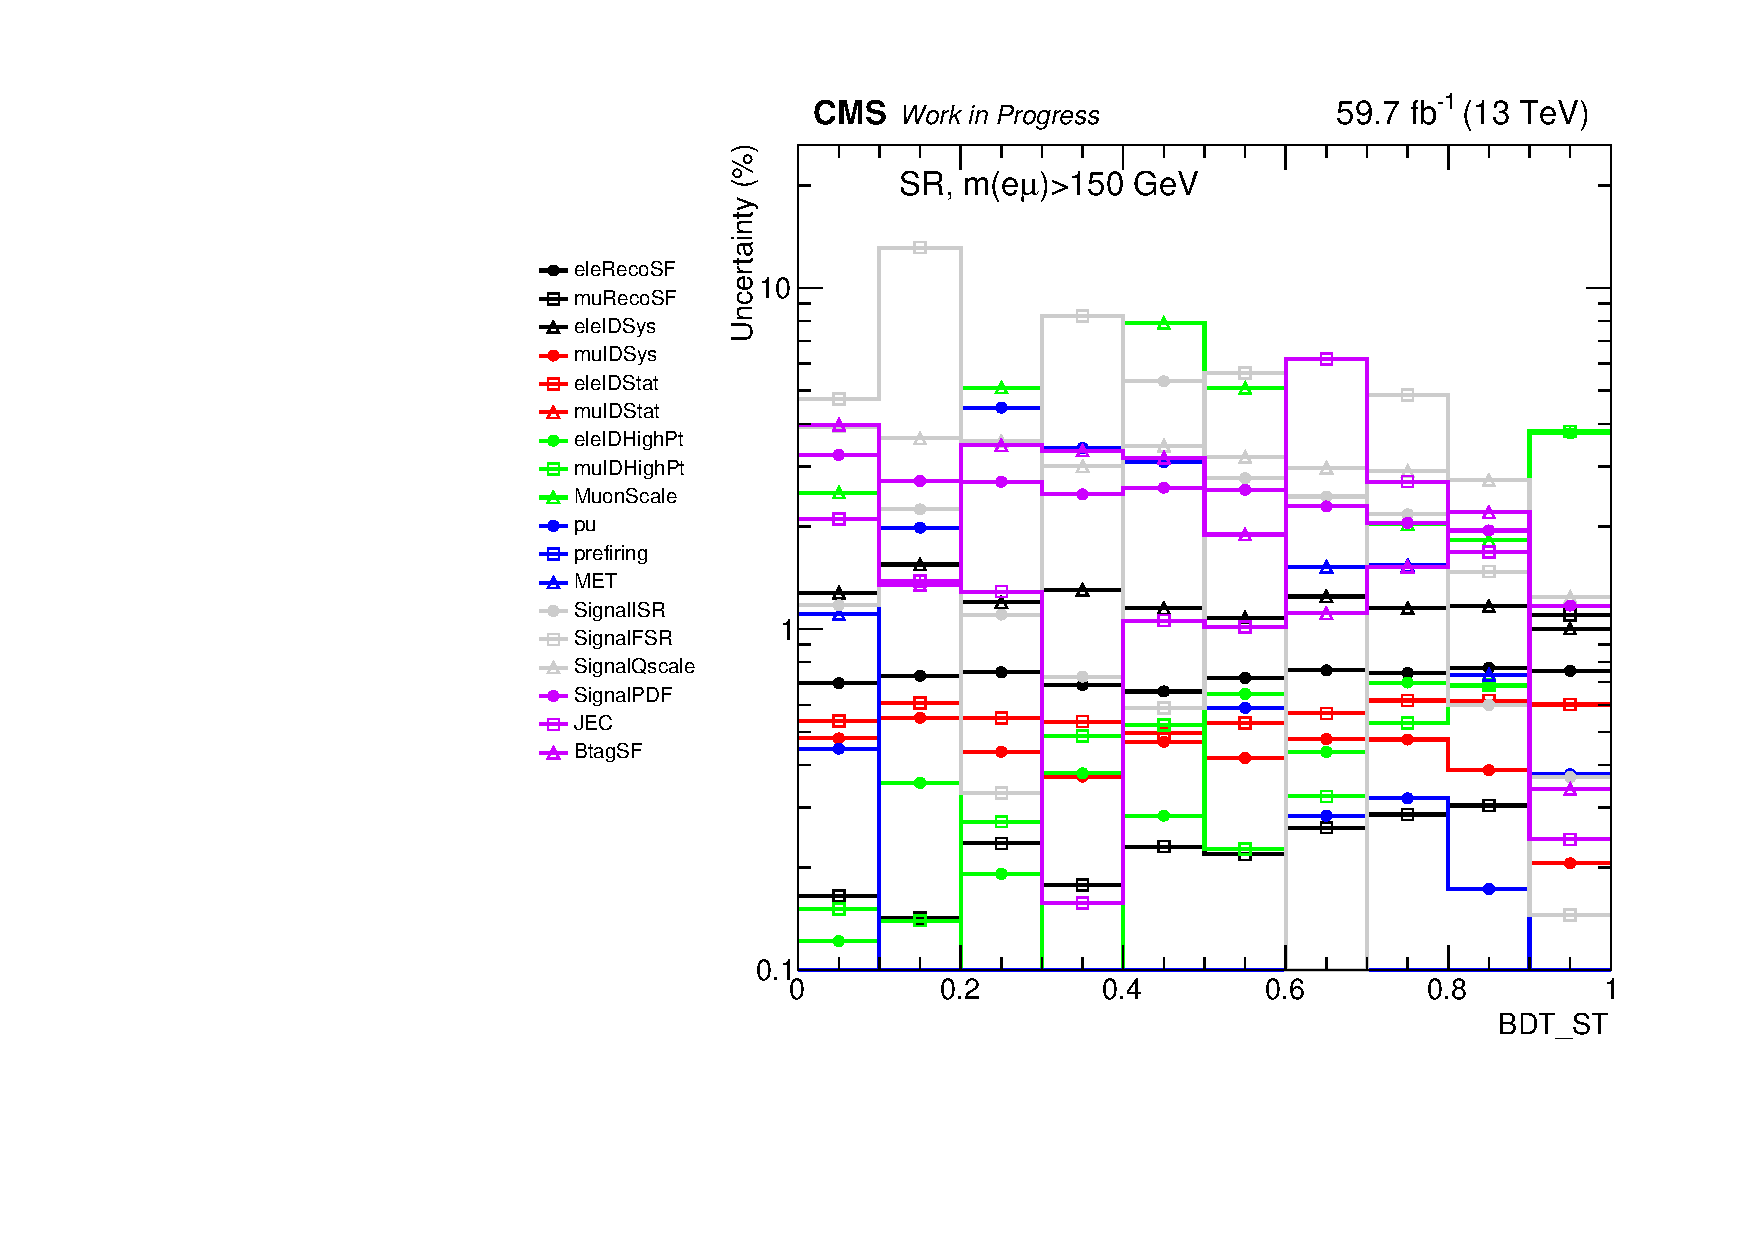
\includegraphics[width=0.45\textwidth]{figures/Part3/Systematics/sysBDT_ST_sig_2018}&
  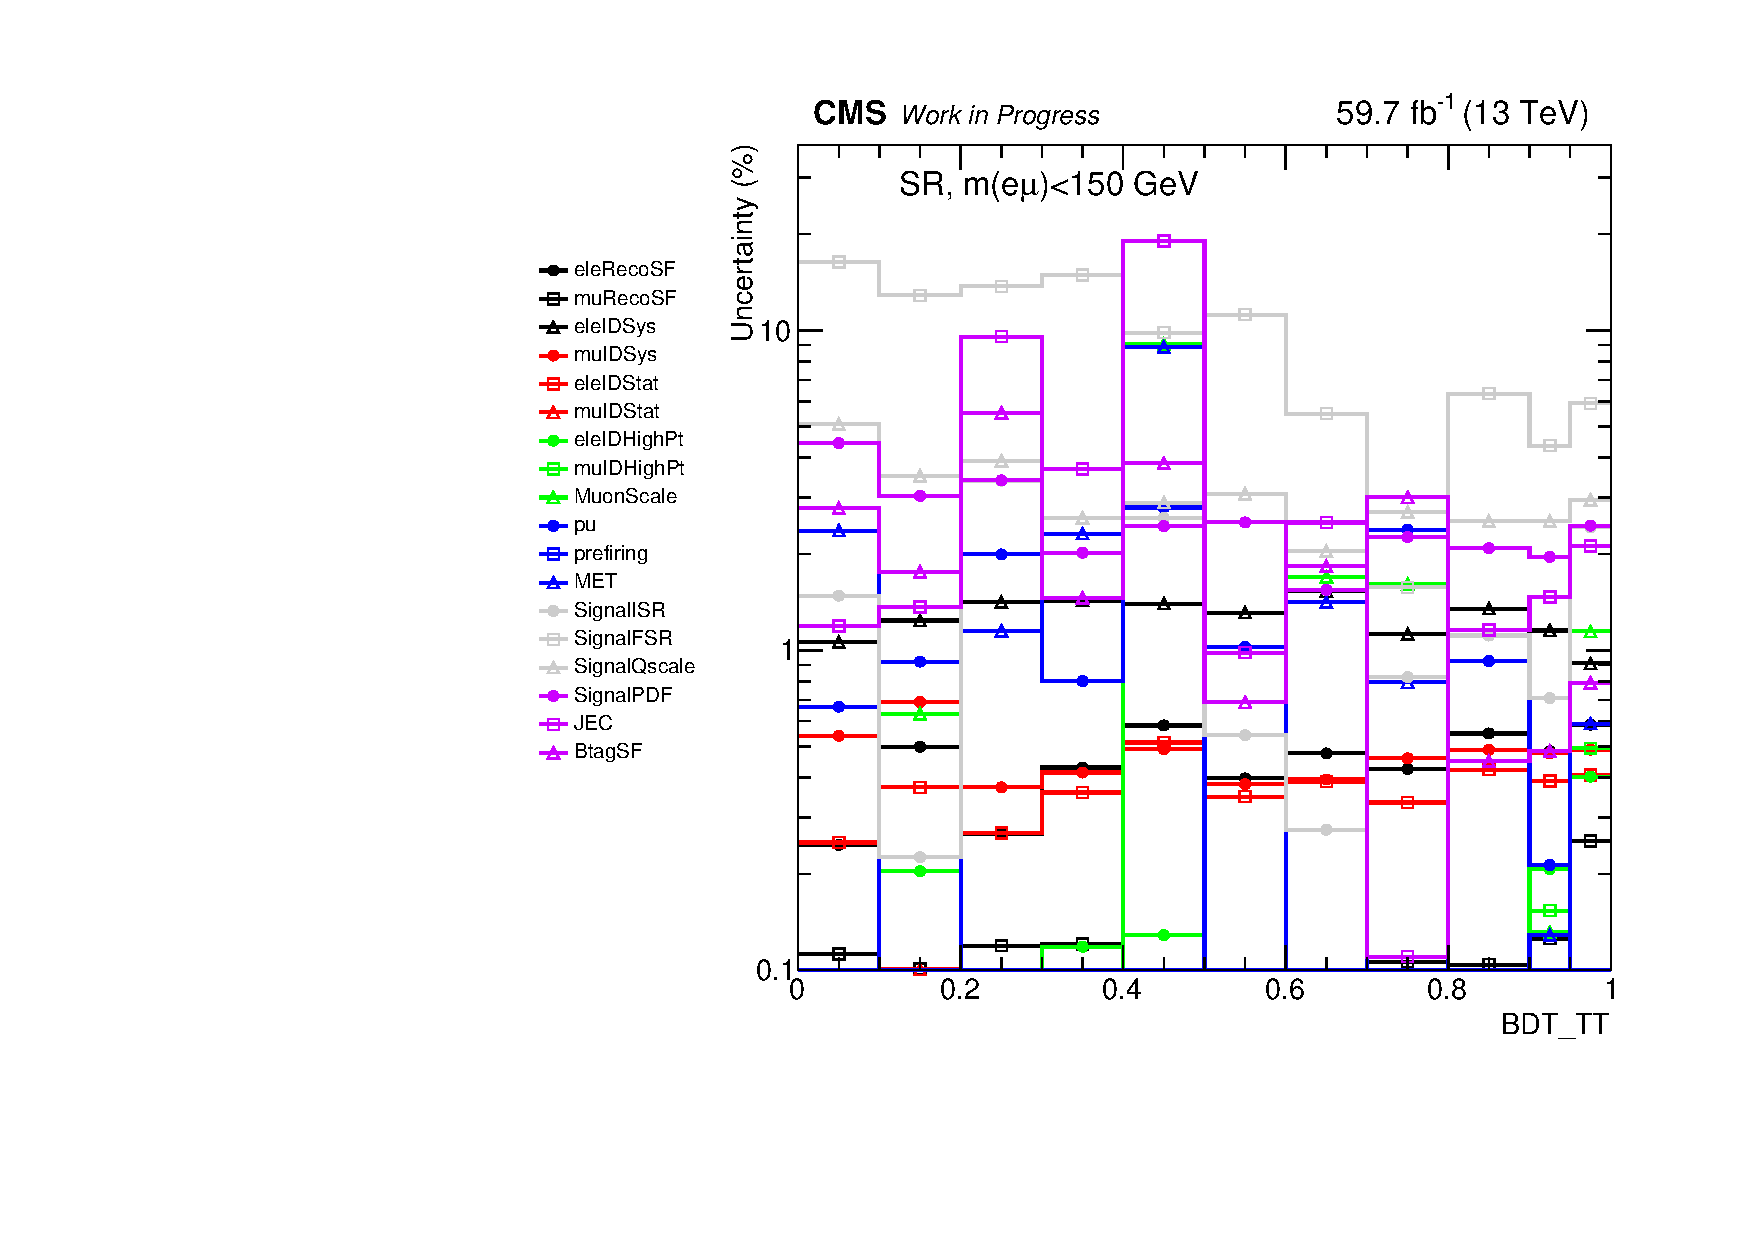
\includegraphics[width=0.45\textwidth]{figures/Part3/Systematics/sysBDT_TT_sig_2018} \\
 \end{tabular}
 \caption{Distributions of relative uncertainties on signal ($C_{e\mu tu}^{vector}$ is used as an example) as a function of BDT output in ST enriched SR (left), TT enriched SR (right). Luminosity and normalization uncertainties are not included in these plots. JES, JER and HEM are combined into "JEC". Sources of b-tagging uncertainties listed in Table~\ref{tab:btag} are combined into "BtagSF". From top to bottom: 2016, 2017 and 2018 datasets.}
 \label{fig:Comp_sys_signal}
 \end{center}
\end{figure}

Representative range of systematic uncertainties on background and signal MC samples are summarized in cite{SysError}. These uncertainties are extracted from the last bins of the BDT distribution.